As we found in \autoref{section: TOV equation}, the Tolman-Oppenheimer-Volkoff equation, \autoref{TOV}, determines the pressure as a function of the radius of a star given the equation of state and the central pressure.
From \autoref{chapter: thermodynamics}, we have various equations of state for the pion condensate.
In this chapter, we will apply these results to study pion stars, bosonic stars composed of a gravitationally bound pion condensate.



\section{Units and limiting radius}

We can gain some insights by reviewing the characteristic quantities of the problem.
The characteristic mass and length, as discussed in \autoref{section: TOV equation}, are found by setting $k_1 = k_2 = k_3 = 1$.
These are the dimensionless constants of the TOV equation, \autoref{dimensionless constants TOV}.
At leading order, the bare constants $f$ and $\bar m$ are related to physical constants by $f = f_\pi$ and $m = m_\pi$, the pion decay constant and the pion mass.
Using the values for $f_\pi$ and $m_\pi$ as given in \autoref{section: units} and reinstating $c$ and $\hbar$, these quantities are given by
%
\begin{align}
    u_0 & =m_\pi^2 f_\pi^2 \frac{c}{\hbar^3}
    = 3.216\cdot 10^{33} \, \text{J}\,\text{m}^{-3}, \\
    m_0 & = \frac{c^4}{\sqrt{\frac{4 \pi}{ 3} u_0 G^3}} = 64.21\, M_\odot, \\
    r_0 & = \frac{G}{c^2} m_0 = 94.79 \, \text{km}.
\end{align}
%
We expect a pion star made up of a pure pion condensate to have dimensions of this order of magnitude, around one order of magnitude larger than the star made up of cold neutrons.
However, when we introduce leptons there is not just one characteristic energy scale, and it becomes harder to anticipate the scale of the stars.



In \autoref{section: thermodynamics leading order}, we found that the leading order, the non-relativistic limit of the equation of state of a pure pion-condensate, without electromagnetic interaction, is $\tilde p =8^{-1} \tilde u^2$.
That is, it is a polytrope with $\gamma = 2$.
As discussed in \autoref{subsection: Newtonian limit and polytropes}, this corresponds to a situation where the radius of the star is independent of the central pressure, at least in the Newtonian limit of gravity.
When simulating the Newtonian, non-relativistic limit of the pion star, we should expect the radius to be constant.
From \autoref{Radius polytrope}, the radius is $R = C \xi_1$, where
%
\begin{equation}
    C = \frac{1}{\sqrt{4(4\pi ) G u_0}} = \frac{1}{\sqrt{12}}r_0,
\end{equation}
%
and $\xi_1$ is the root of the Lane-Emden function $\theta(\xi)$ for polytrope index $n=1$, the solution to
%
\begin{equation}
    \theta'' + \frac{2}{\xi} \theta' + \theta = 0.
\end{equation}
%
By substituting $\theta$ for its power series expansion, $\theta = \sum_n a_n \xi^n$, we get
%
\begin{equation}
    \sum_n \left[ (n+2)(n+1) a_{n+2} + 2(n+1) a_{n+1} \xi^{-1} + a_n \right] \xi^n = 0.
\end{equation}
%
This must be obeyed for arbitrary $\xi$.
We therefore get the recursion relation $a_{n+2} = - a_n / (n+1)(n+2)$.
With our boundary conditions, the solution is
%
\begin{equation}
    \theta(\xi) = \frac{\sin(\xi)}{\xi},
\end{equation}
%
and the first root is therefore $\xi_1 = \pi$.
With this, we get a closed-form expression for the stellar radius of this non-relativistic and Newtonian limit---which we expect the full theory to approach as the central pressure decreases---namely
%
\begin{equation}
    \label{radius pion star nr limit}
    R = \frac{\pi}{\sqrt{12}} r_0 = 85.97 \, \text{km}.
\end{equation}
%
When including electromagnetic interactions, as done in \autoref{subsection: including electromagnetism lo eos}, the non-relativistic equation of state remains a polytrope with $\gamma=2$, however with a new constant by a factor $(1+\Delta)^2$, where $\Delta = \Delta m^2_\text{EM}/m_\pi^2$.
This affects the limiting radius, which now is
%
\begin{equation}
    \label{maximum mass pion star with em interaction}
    R = \frac{\pi}{\sqrt{12}(1 + \Delta)} r_0 = 80.40 \, \text{km}.
\end{equation}
%
These limits are only available when considering the pion condensate alone, without leptons.
As we found, the inclusion of leptons will change the low-density limit of the equation of state, and it is only for $\gamma=2$ where the Lane-Emden equation admits a finite limit radius of this sort.



\section{Leading order results}

In this section and the next, we present the results of numerically integrating the TOV equation using the various equations of state we have obtained.
The computer code used to obtain these results is discussed in \autoref{appendix: code}.



\subsection{Pion star of pure pion condensate}

We start with the simplest case of a pure pion condensate, in which there are only strong interactions, to leading order as described in \autoref{subsection: pure pion condensate}.
The equation of state of this system is shown in \autoref{fig: equation of state pions}.
\autoref{fig: pressure and mass for pion star} shows the pressure and mass as a function of radius for varying values of central pressure.
The quantities are normalized to the central pressure, stellar mass, and stellar radius, respectively.
The black dashed line corresponds to the configuration with the maximum mass.
We see that both the pressure and mass distribution are very similar for stars with a mass less than the maximum.
As the central pressure increase beyond that of the star with maximum mass, the pressure close to the center grows sharply.
This is similar to what we saw in the case of an incompressible fluid, \autoref{subsection: incompressible fluid}.

\autoref{fig: mass-radius relation pion star} shows the mass-radius relation for the pion star.
As in the case of the neutron star it has a maximum mass, $M_\text{max} = 10.47\, M_\odot$, and a corresponding radius $R = 55.44\,\text{km}$.
However, in contrast to the case of the neutron star, the stellar radius approaches a maximum radius as the central pressure decreases.
This matches our expectation from the non-relativistic, Newtonian limit.
We see that the largest radius in our results, corresponding to  $p_c = 10^{-6} \, p_0$, is $R = 85.91 \, \text{km}$, an excelent fit with our earlier analysis, \autoref{radius pion star nr limit}.
\autoref{fig: mass-radius relation pion star comparison} compares the mass-radius relation from the full equation of state and TOV equation with various limits.
In the non-relativistic, Newtonian limit, the stellar radius is independent of the mass, as we found in our earlier analysis.


\begin{figure}[H]
    \centering
    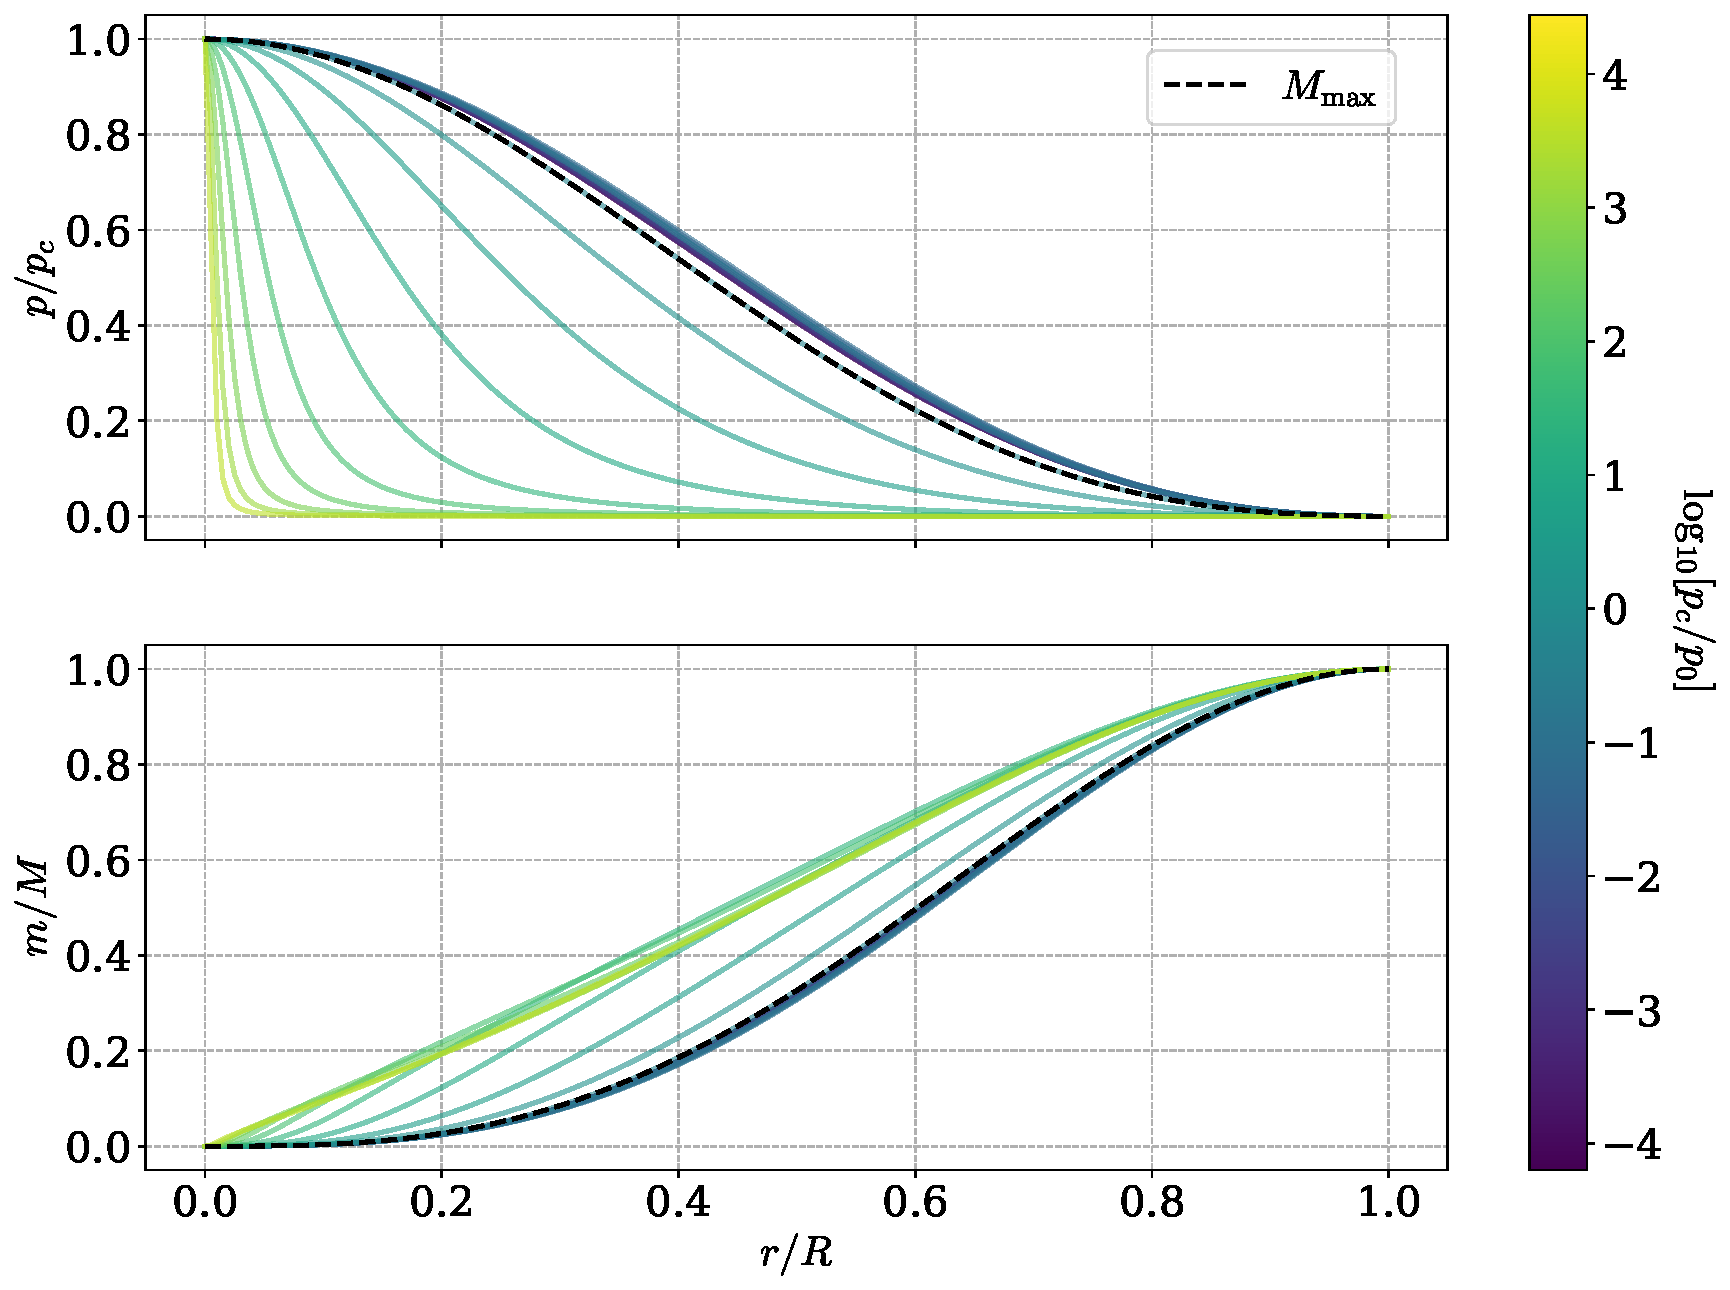
\includegraphics[width=.85\textwidth]{../scripts/figurer/pion_star/pressure_mass_pion_star.pdf}
    \caption{
    Top: The pressure normalized to the central pressure.
    Bottom: The mass, normalized to the stellar mass.
    Both are functions of radius $r$, normalized to the stellar radius, and the plots show a range of stars with different central pressures, indicated by the color.
    The black dashed line corresponds to the star with the largest mass.
    }
    \label{fig: pressure and mass for pion star}
\end{figure}

\begin{figure}[H]
    \centering
    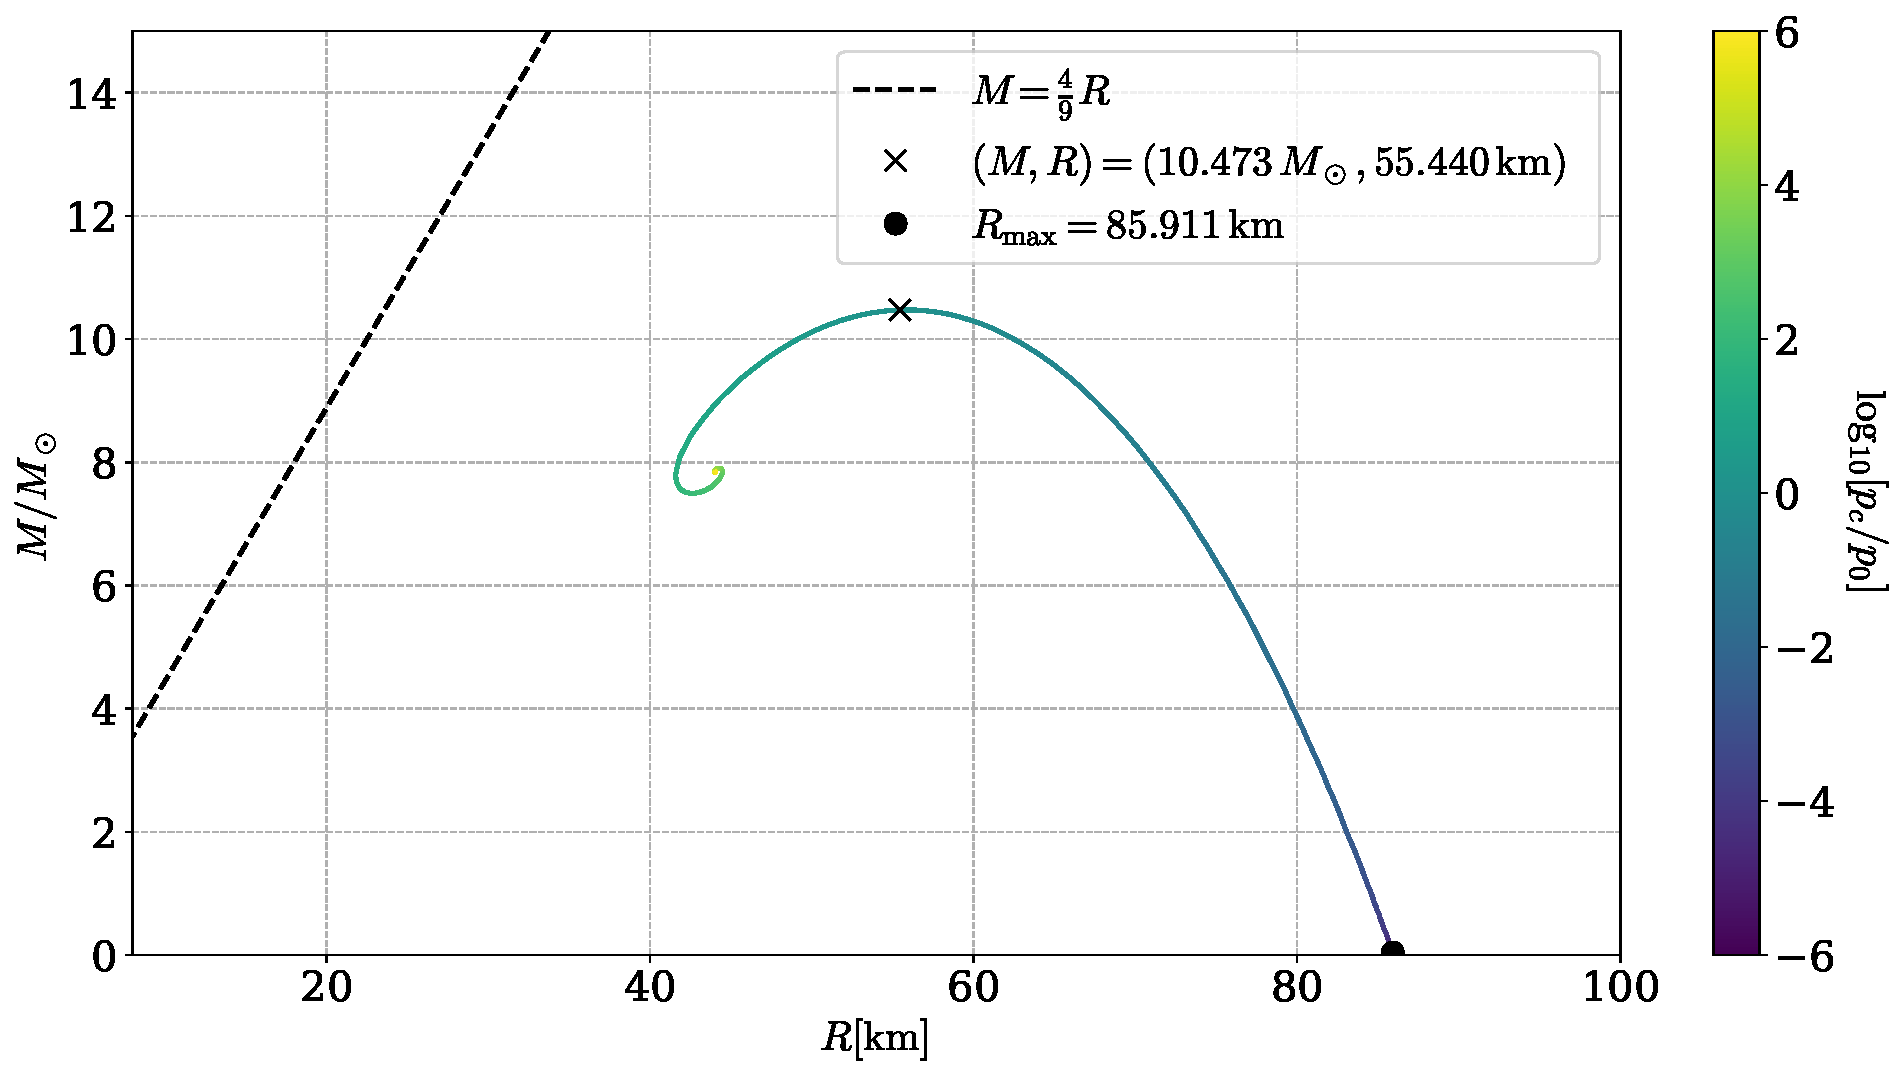
\includegraphics[width=0.85\textwidth]{../scripts/figurer/pion_star/mass_radius_pion_star.pdf}
    \caption{
        The mass-radius relation of a pion star of a pure pion condensate, to the lowest order using \chpt.
        The mass is given in units of solar masses, while the radius is measured in kilometers.
        This line is parameterized by the central pressure $p_c$ of the star, as indicated by the color gradient.
        The dashed black line indicates the theoretical maximum mass for a given radius, and any configuration above it will collapse to form a black hole.
        }
        \label{fig: mass-radius relation pion star}
\end{figure}

\begin{figure}[H]
    \centering
    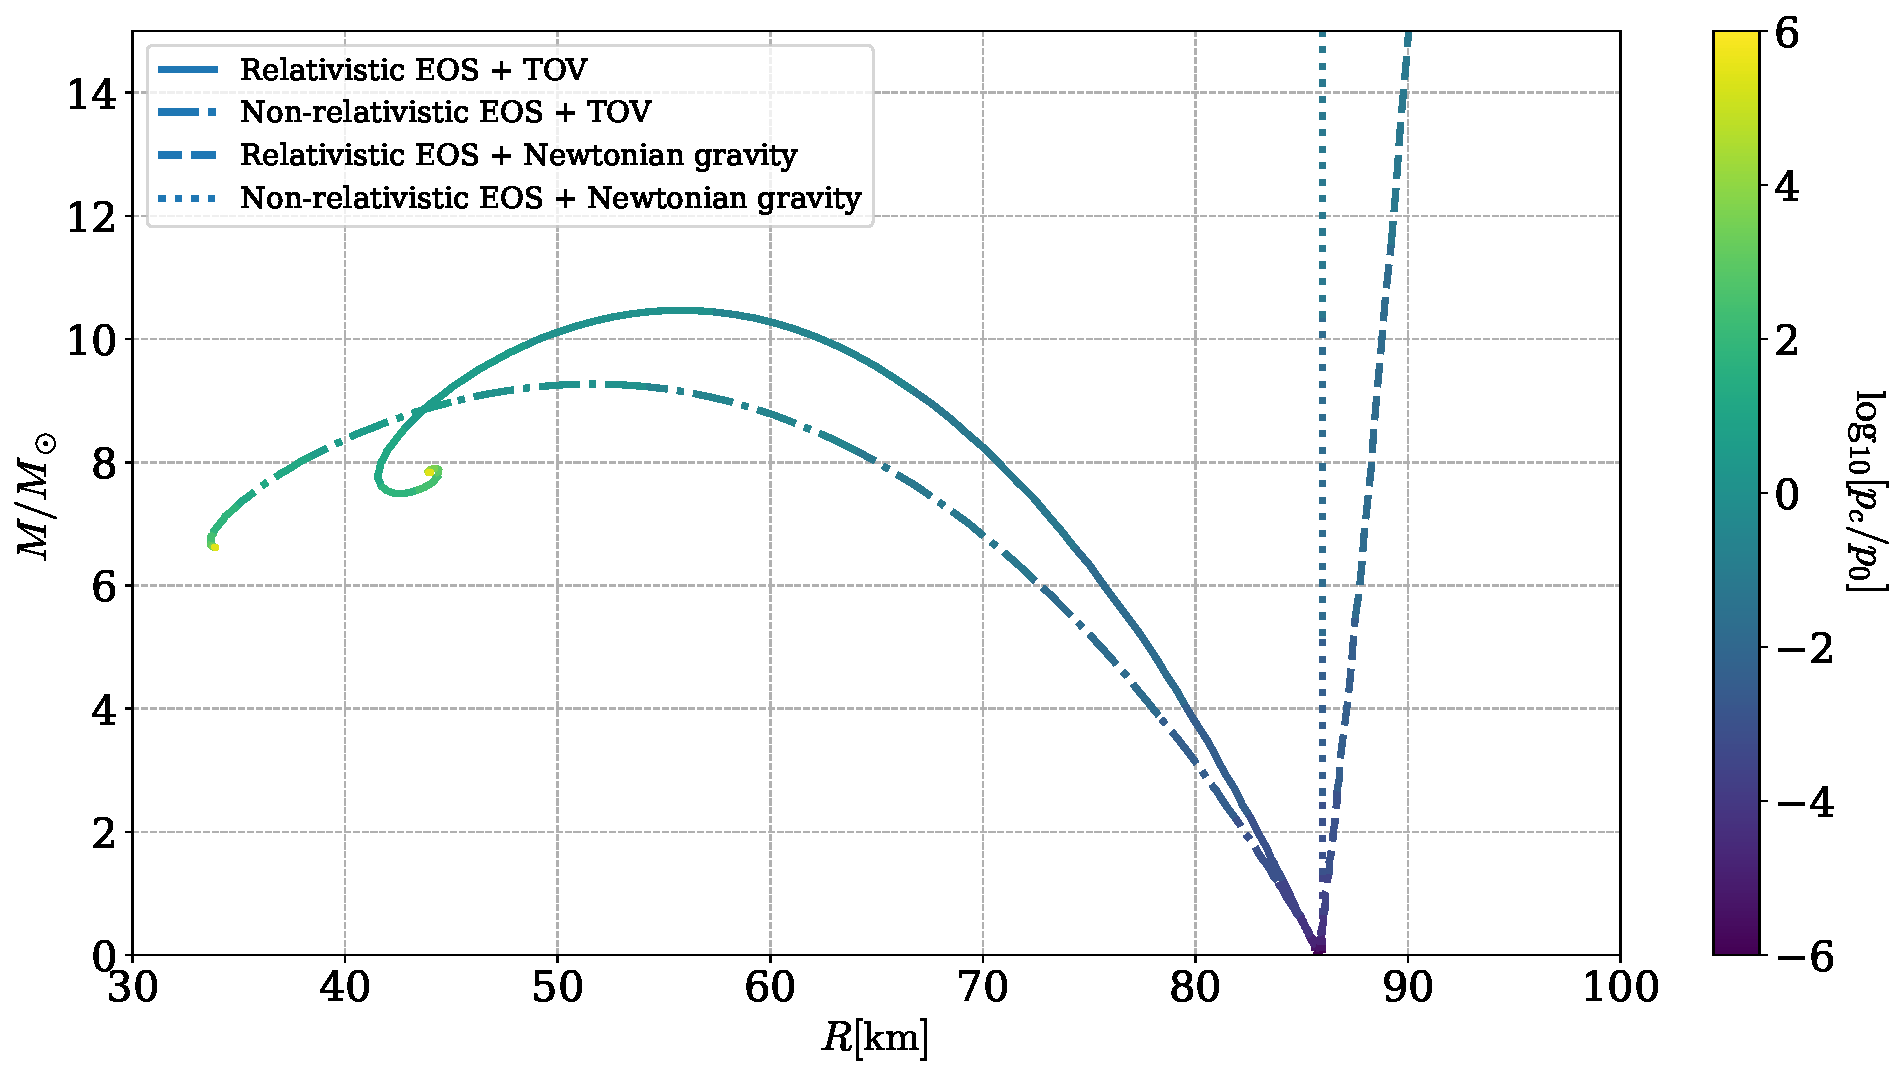
\includegraphics[width=0.85\textwidth]{../scripts/figurer/pion_star/mass_radius_comparison.pdf}
    \caption{
        The mass-radius relationship of the pion star using the full, leading-order equation of state from \chpt\, and the TOV equation, compared with results in various limits.
        }
        \label{fig: mass-radius relation pion star comparison}
\end{figure}




\subsection{Including electromagnetic contributions}

As we found in \autoref{subsection: including electromagnetism lo eos}, the electromagnetic interaction of the pseudoscalar mesons contributes to the equation of state, even at leading order.
\autoref{fig: pressure and energy with EM interaction} shows the pressure and energy density, normalized to their characteristic quantities, as a function of chemical potential above the critical value, normalized to $m_\pi$.
\autoref{fig: eos chpt em interaction} shows the equation of state.
The results with and without electromagnetic results are compared.
We see that the inclusion of electromagnetic contributions results in a less stiff equation of state; a given pressure corresponds to a higher energy density when including electromagnetic interactions.
\autoref{fig: mass-radius relation comparison} shows the mass-radius reaction of the pion star when the electromagnetic interaction is taken into account and compares it with our earlier result.
We see that the shape of the curve has not changed much from the earlier result. 
Both the maximum mass and radius are slightly smaller.
As discussed in \autoref{section: cold fermi star}, we expect a stiffer equation of state to correspond to a more massive star, as happens in this case.
The new result for maximum radius, $R = 80.40 \, \text{km}$, is in excellent agreement with our expectation, \autoref{maximum mass pion star with em interaction}.


\begin{figure}[H]
    \centering
    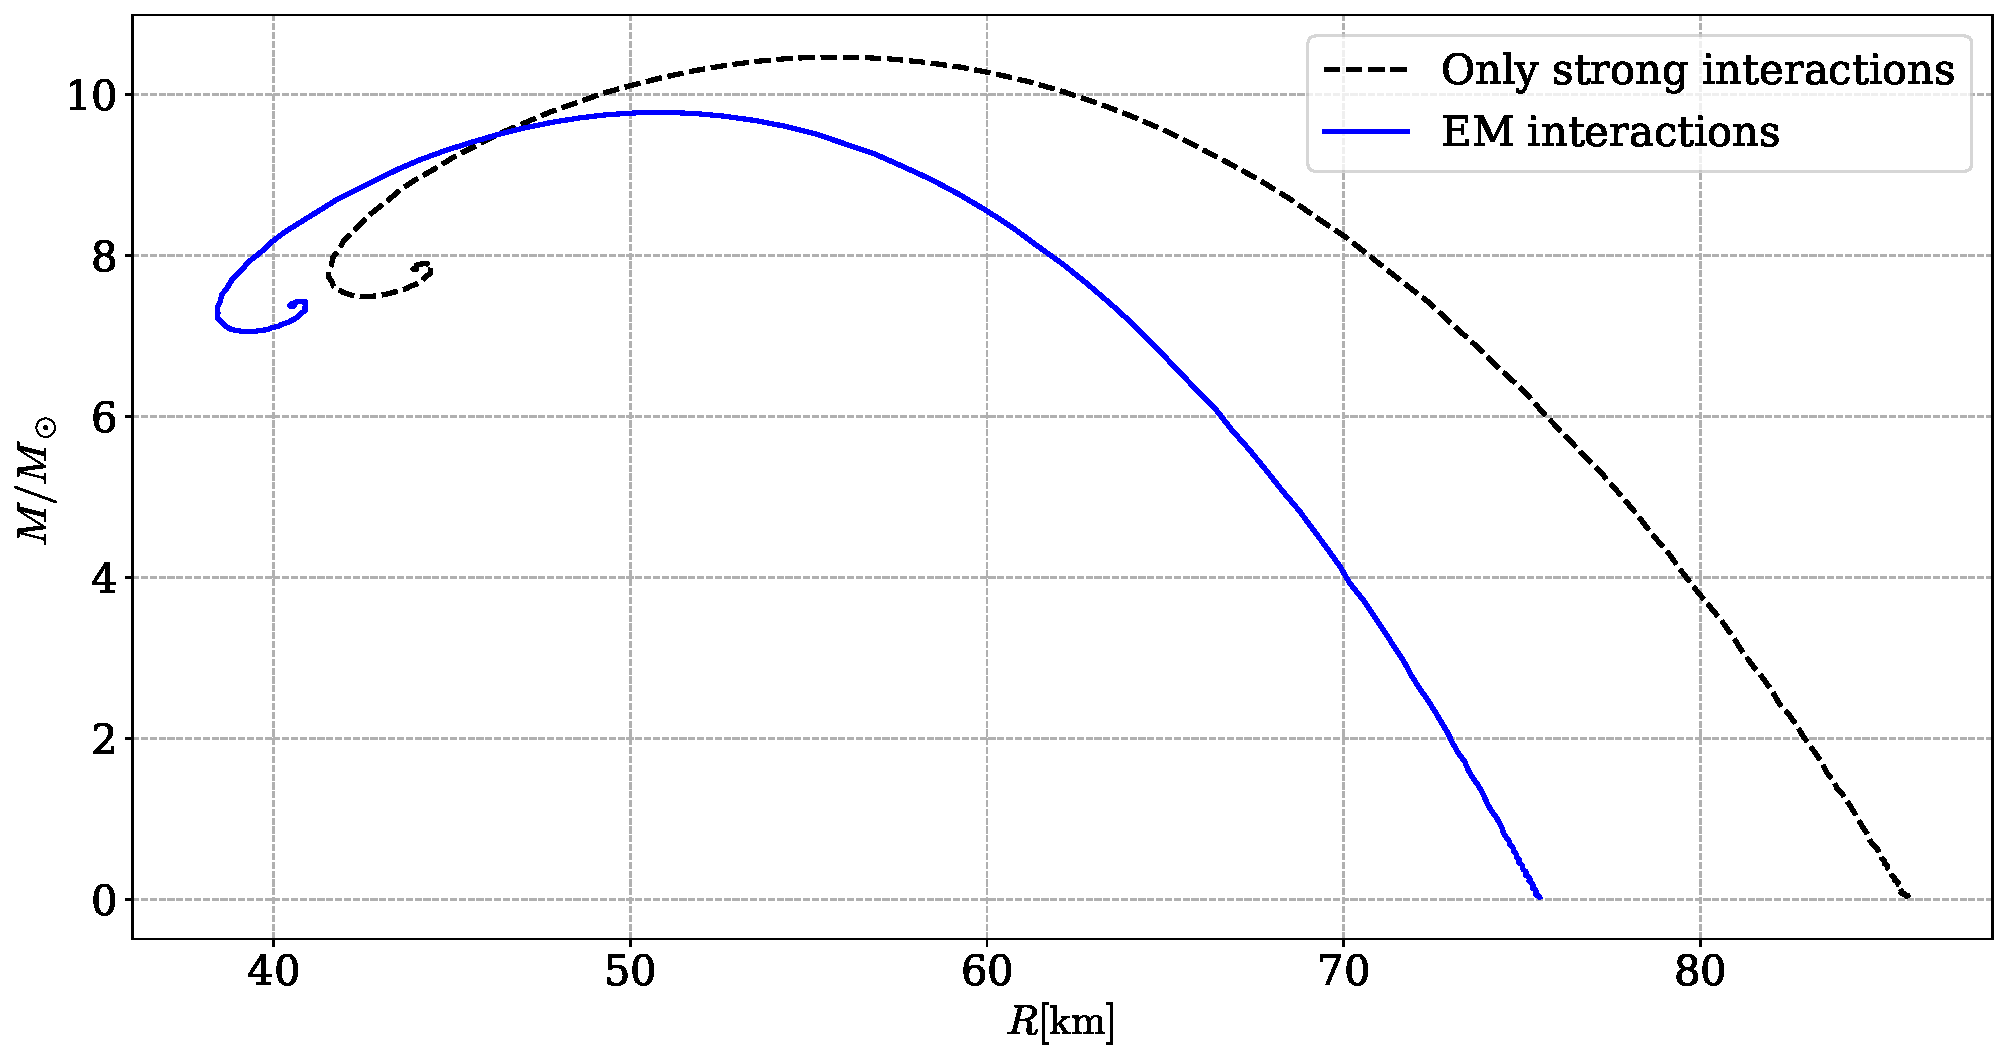
\includegraphics[width=0.75\textwidth]{../scripts/figurer/pion_star/mass_radius_pion_star_compare.pdf}
    \caption{
        The mass-radius relation of pion stars with and without the effects of electromagnetism.
        The mass is in units of solar masses, the radius in kilometers.
        The marked points are the maximum mass and corresponding radius of the stars.
        }
        \label{fig: mass-radius relation comparison}
\end{figure} 




\subsection{Charge neutral stars}


We now apply the results from \autoref{section: charge neturality}, where we added a lepton to enforce charge neutrality.
As the electromagnetic force is long-range, we should expect any macroscopic astronomical object to be charge neutral.
First, we apply the system of pions and one charged lepton.
The star with electrons is shown in \autoref{fig: mass-radius relation with electrons}.
We see that this star is much larger than those made of only pions.
This is because the light electrons make the equation of state stiffer at low pressures.
The non-relativistic equation of state is now a polytrope with $\gamma = \frac{5}{3}$, instead of $\gamma = 2$, and there is no upper limit on the radius.
The maximum mass is now $239\, M_\odot $, and the corresponding maximum radius is $ 3.2\times10^4\,\text{km}$.

The mass-radius relation for a star where the lepton is a muon is shown in \autoref{fig: mass-radius relation with muons}.
This has a similar form to the one with the electron, only smaller and lighter, as the equation of state, in this case, is less stiff.
The maximum mass is now $18.6\, M_\odot $, and the corresponding maximum radius is $ 262 \,\text{km}$.

\begin{figure}[H]
    \centering
    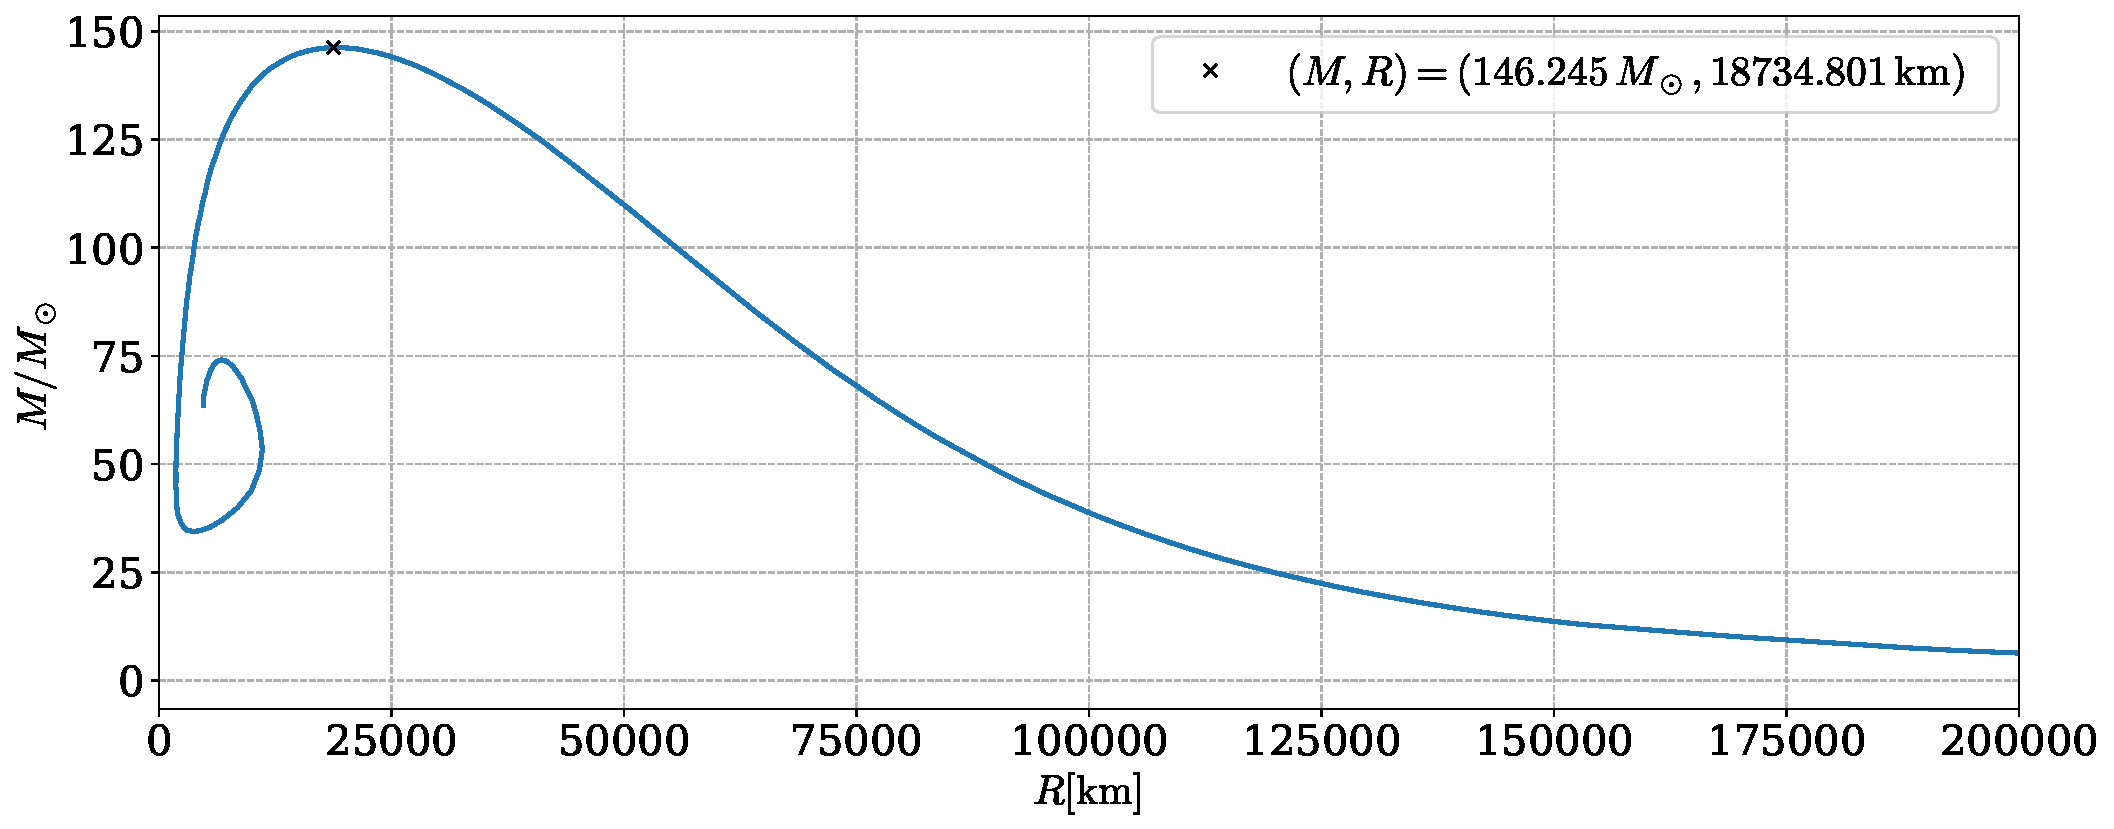
\includegraphics[width=.85\textwidth]{../scripts/figurer/pion_star/mass_radius__e.pdf}
    \caption{
        The mass-radius relation of pion stars, including electrons to enforce charge neutrality, is parameterized by the central pressure.
        The mass in units of solar masses, the radius in kilometers, and the pressure in $p_0 = f_\pi^2 m_\pi^2$.
        }
        \label{fig: mass-radius relation with electrons}
\end{figure}

\begin{figure}[H]
    \centering
    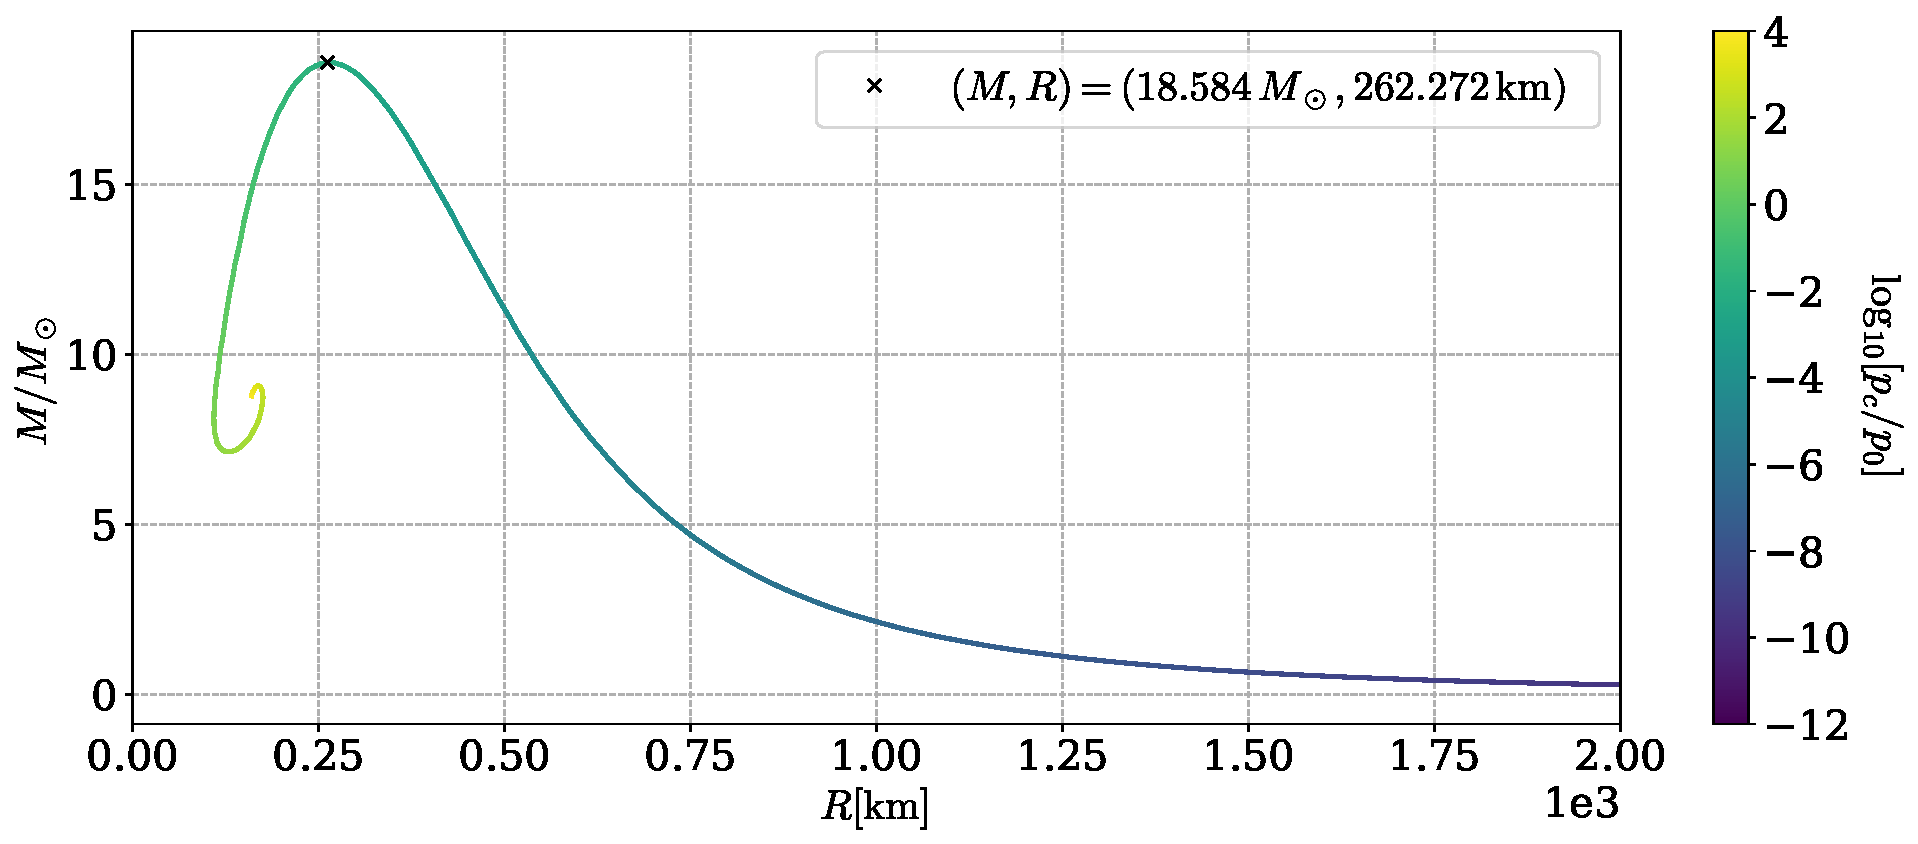
\includegraphics[width=.85\textwidth]{../scripts/figurer/pion_star/mass_radius__mu.pdf}
    \caption{
        The mass-radius relation of pion stars, including muons to enforce charge neutrality, is parameterized by the central pressure.
        The mass in units of solar masses, the radius in kilometers, and the pressure in $p_0 = f_\pi^2 m_\pi^2$.
        }
        \label{fig: mass-radius relation with muons}
\end{figure}




\subsection{Neutrinos}

As discussed in \autoref{subsection: neutrinos}, a more realistic charge-neutral pion condensate includes weak decay, in which case both electrons and muons will be present and in chemical equilibrium with their respective neutrinos.
The resulting equation of state is illustrated in \autoref{fig: neutrino eos}.
As the neutrino contribution is dominating, this equation of state is close to the $u = 3p$ equation of state of ultrarelativistic fermions.
Below the point where the pion condensate vanish, at $p = p_\text{min}>0$, the equation of state is exactly $u = 3p$.
In terms of the characteristic quantitites, the minimum pressure is $p_\text{min} = 1.84 \times 10^{-2} u_0$.
A star with $u = 3p$ will not have a finite radius where the pressure vanishes.
However, as the isospin density vanish at $p = p_\text{min}$, we define the stellar radius $R$ by $p(R) = p_\text{min}$.
Such a star will therefore have an atmosphere of ultrarelativistic neutrinos.
There is a $p+u$-term on the right-hand side of the TOV equation, \autoref{TOV}.
When we defined the stellar radius by $p(R) = 0$, this factor vanishes as we approach the surface of the star, while now $p+u \geq 4 p_\text{min}$ at all radii.
Close to the surface, the pressure will therefore fall faster, as a consequence of $p_\text{min}>0$.
The resulting mass-radius relation is shown in \autoref{fig: mass radius neutrino}.
We see that, in contrast to the earlier results, both the mass and radius approach zero as $p_c \rightarrow p_\text{min}$.
The maximum mass is now $M_\text{max} = 18.8 M_\odot$, with a corresponding radius $R = 125 \, \text{km}$.
At the bottom of \autoref{fig: mass radius neutrino}, the pion stars including charged leptons and neutrinos are compared to a family of stars with $u = 3p$ but different values for $p_\text{min}$.
As $p_\text{min}$ increases, the mass-radius relation is scaled down.
As the $p_\text{min}$ approaches zero, the maximum mass will diverge.
We see that the mass-radius relation of the pion star closely resembles that of such a star.
The mass-radius relationship, therefore, is mostly set by $p_\text{min}$.
The equation of state of the $\pi\ell\nu_\ell$-system is somewhat less stiff than $u = 3p$, at least for central pressures below that of the maximum mass star, and we see that the result is a smaller and lighter star for the same value of $p_\text{min}$.

\begin{figure}[H]
    \centering
    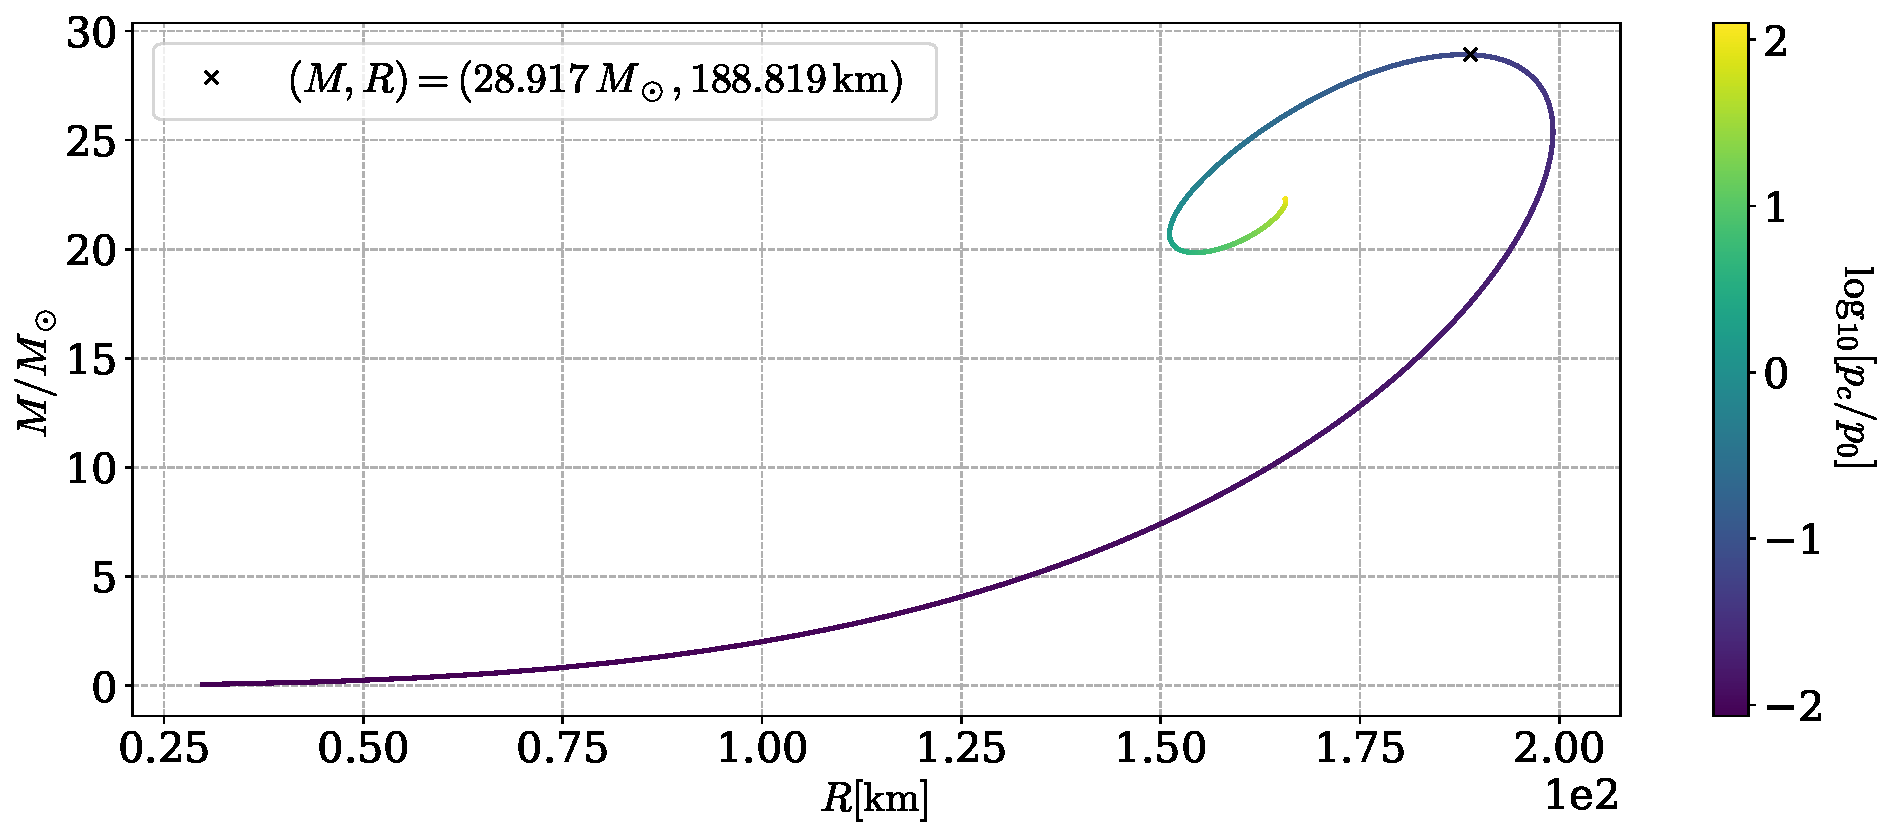
\includegraphics[width=.8\textwidth]{../scripts/figurer/pion_star/mass_radius_neutrino.pdf}
    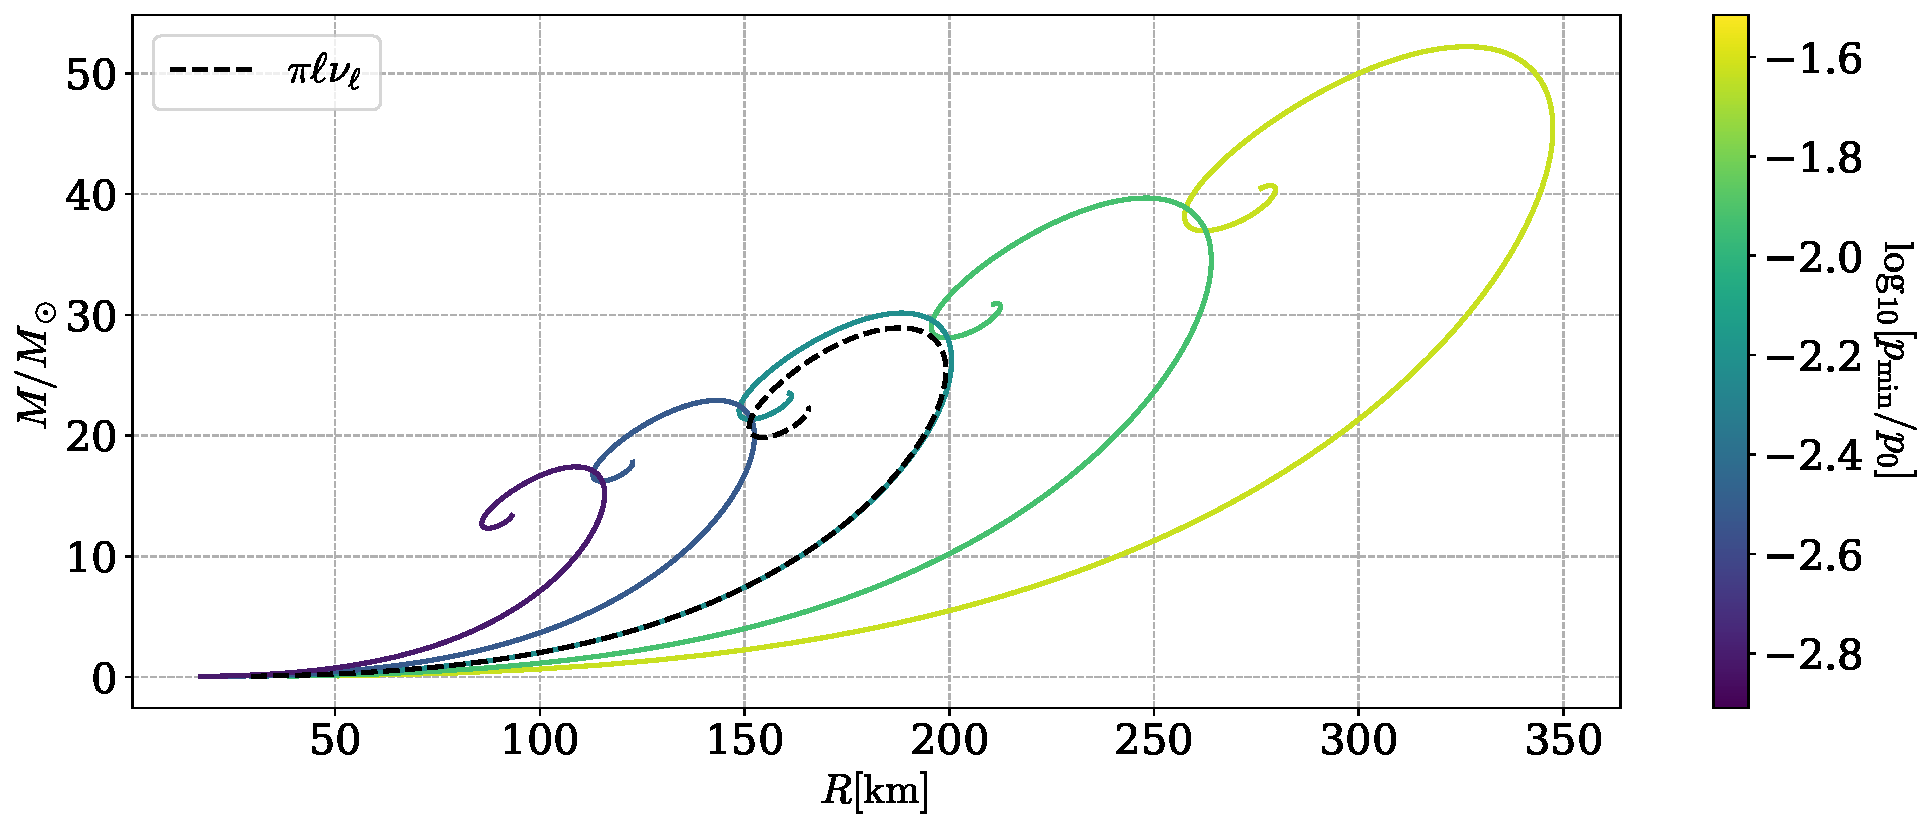
\includegraphics[width=.8\textwidth]{../scripts/figurer/pion_star/mass_radius_light.pdf}
    \caption{
        The mass-radius relation of pion stars, including leptons and neutrinos in equilibrium.
        The radius is given in kilometers and the mass in units of solar masses.
        Top: The full $\pi\ell\nu_\ell$-system, whit maximum mass marked by a cross.
        Bottom: The $\pi\ell\nu_\ell$-system is compared to results using $u=3p$, and different values of $p_\text{min}$
        }
        \label{fig: mass radius neutrino}
\end{figure}



\section{Next-to-leading order results}

In \autoref{section: nlo thermodynamics}, we calculated the NLO free energy of the pion condensate, and with this, we found the NLO equation of state of the pure pion condensate as well as the $\pi\ell\nu_\ell$-system.
We now use these equations of state to obtain the corresponding NLO mass-radius relations.
\autoref{fig: mass-radius relation compare nlo} shows the NLO mass-radius relation of a pion star composed of a pure pion condensate and compares it to the LO result.
The results are similar, however, the next-to-leading order star is smaller and less massive, as is expected for a less stiff equation of state.
The maximum mass of the NLO star is $M_\text{max} = 9.64\, M_0$, and the corresponding radius is $R = 54.09\,\text{km}$.

The NLO mass-radius relation of pion stars including charged leptons and neutrinos are shown in \autoref{fig: mass-radius relation compare nlo neutrino}.
As discussed in \autoref{section: nlo thermodynamics}, the change in the equation of state from LO to NLO is small, and as a consequence, the difference in the mass-radius relations is too.
However, for $p < 0.1 p_0$, the NLO equation of state is slightly stiffer.
From \autoref{fig: mass radius neutrino}, we see that this is the relevant range for stars with a central pressure less than that of the maximum mass star.
As expected the NLO pion star is therefore slightly larger and more massive.
This relationship is still well approximated by a $u = 3p$ equation of state with some cut-off pressure $p_\text{min}$.

\begin{figure}[H]
    \centering
    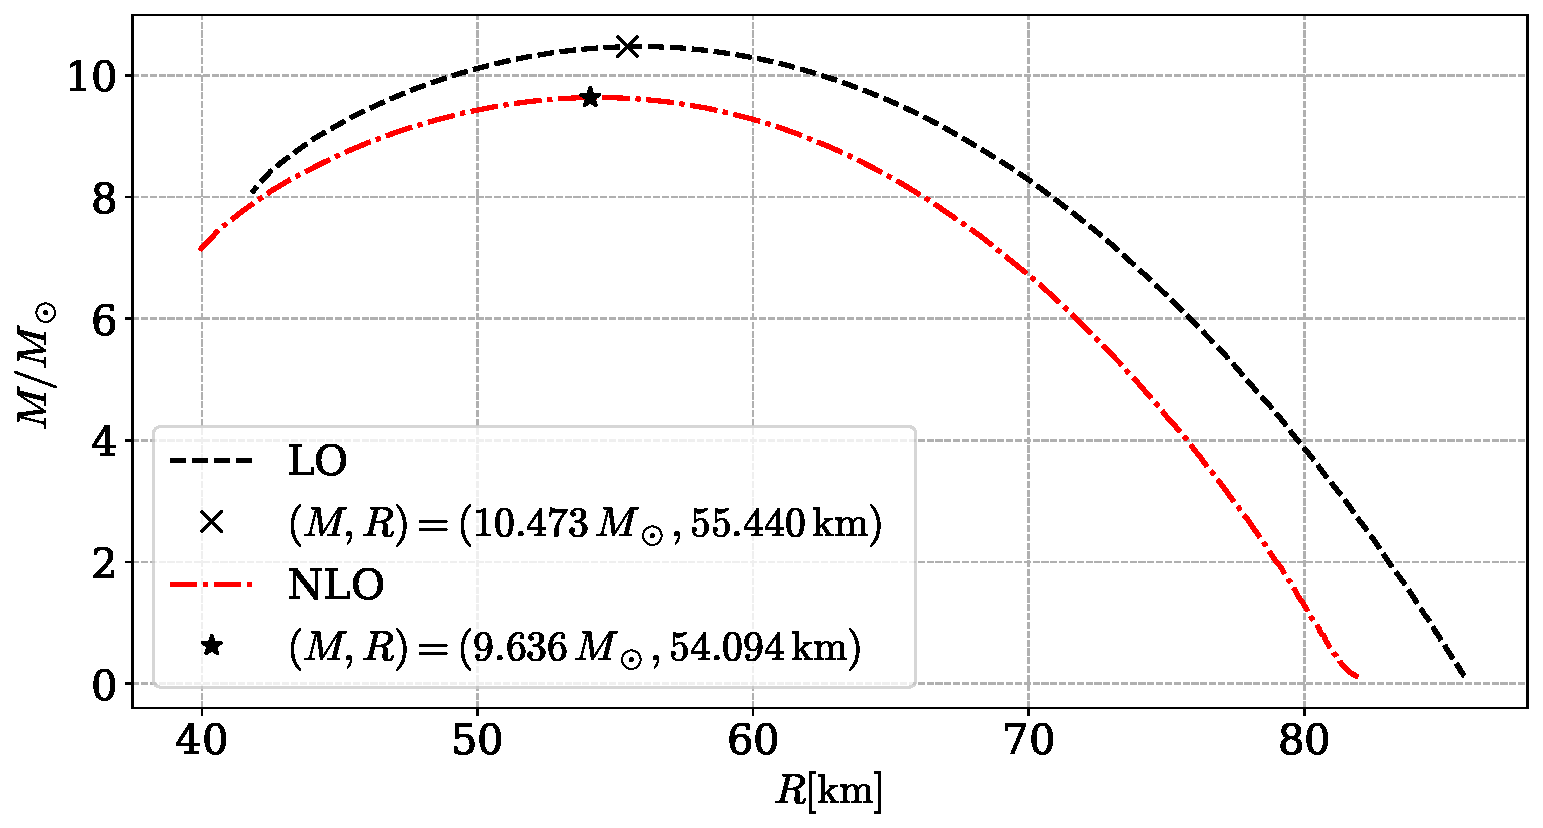
\includegraphics[width=.75\textwidth]{../scripts/figurer/pion_star/mass_compare_order.pdf}
    \caption{
        The LO and NLO mass-radius relation of pion stars composed of a pure pion condensate are compared.
        The mass is given in solar masses and the radius in kilometers.}
    \label{fig: mass-radius relation compare nlo}
\end{figure}

\begin{figure}[H]
    \centering
    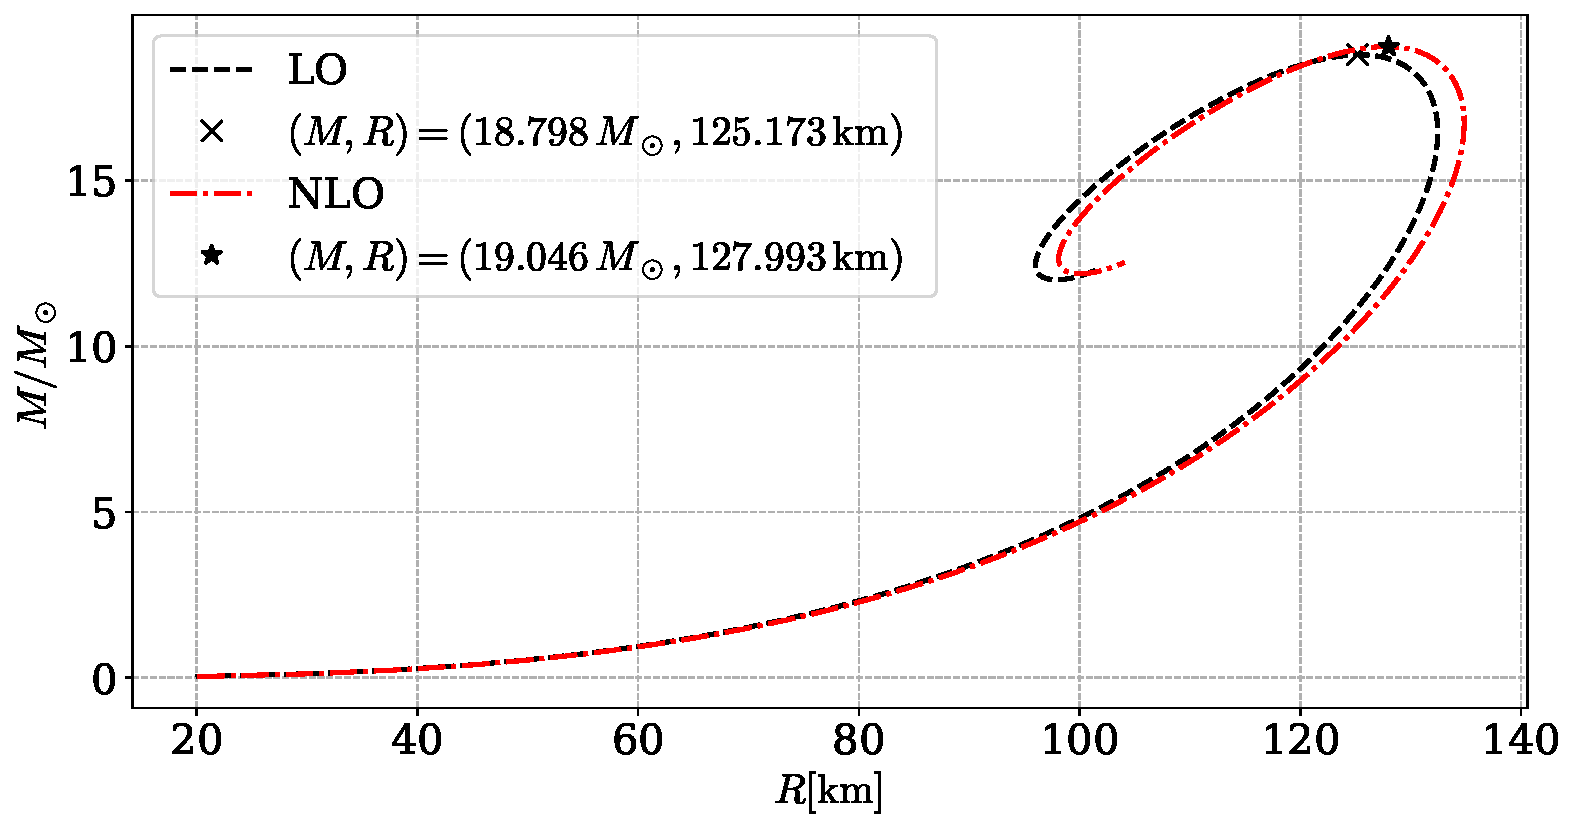
\includegraphics[width=.75\textwidth]{../scripts/figurer/pion_star/mass_compare_order_neutrino.pdf}
    \caption{
        The LO and NLO mass-radius relation of pion stars composed of a pion condensate including leptons and neutrinos are compared.
        The mass is given in solar masses and the radius in kilometers.}
    \label{fig: mass-radius relation compare nlo neutrino}
\end{figure}




\section{Key values and results}

We have modeled pion stars using the equation of state of pion condensates including various effects such as electromagnetism, loop-corrections, charge neutrality and weak interactions.
These various compositions create stars of wildly different sizes and masses.
In this section, we compile the main results.
In \autoref{table: key values} we have combined some key figures for the maximum mass configuration for the different equations of state.
For all the star families, except those of a pion condensate and only electrons, the masses and radii are within an order of magnitude of $m_0$ and $r_0$.
We can explain this by considering that for all these systems, the only energy scales are $f_\pi$, $m_\pi$ and $m_\mu$, which all are close to $100\,\text{MeV}$.
This is true even for the $\pi\ell\nu_\ell$-system, as in this case the energy scale is $p_\text{min}^{1/4}\propto m_\pi$.
The $\pi e$-system, on the other hand, has a different, much lower energy scale, $m_e \approx 0.5 \text{MeV}$, which leads to a corresponding much larger radius and mass for the resulting star.

We see that, for all the different stars, $\mu_I$ is well below the threshold $4\pi f_\pi \approx 8.6 \, m_\pi$ for the convergence of chiral perturbation theory.
The range of validity is somewhat smaller than this, as new degrees of freedom that we have not taken into account come into play.
The lightest particle not in our model is the $\rho$-meson, with mass $m_\rho = 770 \, \text{MeV} \approx 5.7 \, m_\pi$, which is still well above the energies in our result.
For the most realistic composition, the $\pi\ell\nu_\ell$-system, the isospin chemical potential at the center for the maximum mass star is around $0.02\,m_\pi$.
This means that the pion condensate throughout this star, and all those with a lower central pressure, is only slightly above the point of phase transition.

In \autoref{fig: mass-radius relation with leptons} we compare the mass-radius relations of the different stars.
We only include the next-to-leading order result for pure pion condensation and the $\pi \ell \nu_\ell$-system.
This is a logarithmic plot, as both the masses and radii vary over several orders of magnitude.
\autoref{fig: max pressure and mass} shows the mass and pressure distributions of the maximum mass configurations of the various stars.
Among the mass distributions, the $\pi\ell\nu_\ell$-system stands out as the mass increases in a straight line, as opposed to the other distributions, which taper off towards the surface of the star.
In the bottom plot, we see that the pressure of all the stars approaches $0$ as $r$ approaches $R$ except for the $\pi\ell\nu_\ell$-system which approaches $p_\text{min}>0$.
All stars obey the necessary criterion for stability, as discussed in \autoref{subsection: upper bound and stability}, for central pressures below that of the maximum mass star.
Stability analysis done in \autocite{brandtNewClassCompact2018} shows that, as we expect, the stars are stable in this case.


\begin{table}[H]
    \centering
    \caption{The values of some key quantities for the maximum mass configurations of the various stars.}
    \label{table: key values}
    \begin{tabular}{l  c  c  c  c  c}
        \hline \hline
        system & $M_\text{max}/M_\odot$ & $R / \text{km}$ & 
        $u/u_0$ & $p/u_0$ & $\mu_I/m_\pi-1$ \\
        \hline
        $\pi\, \text{LO}$& 10.48 & 55.47 & 2.865 & 1.318 & 1.100 \\
        $\pi\, \text{NLO}$& 9.64 & 54.09 & 3.020 & 1.139 & 0.9256 \\
        $\pi\, \text{EM}$& 10.11 & 53.57 & 2.930 & 1.318 & 1.116 \\
        $\pi e$& 238.8 & 3.171$\times10^4$ & 
        2.550$\times10^{-6}$ & 1.995$\times10^{-8}$ & 
        6.222$\times10^{-7}$ \\
        $\pi \mu$& 18.58 & 262.3 & 
        0.1411 & 1.202$\times 10^{-2}$ &
        1.732$\times10^{-2}$ \\
        $\pi  \ell  \nu_\ell$& 18.80 & 125.2 &
        0.5399  & 0.1492 &
        2.030$\times10^{-2}$ \\
        $\pi  \ell \nu_\ell\,\text{NLO}$& 19.05 & 128.0 &
        0.4960  & 0.1391 &
        1.801$\times10^{-2}$ \\
        \hline
    \end{tabular}
    \vspace*{3cm}
\end{table}


\clearpage

\begin{figure}[p]
    \centering
    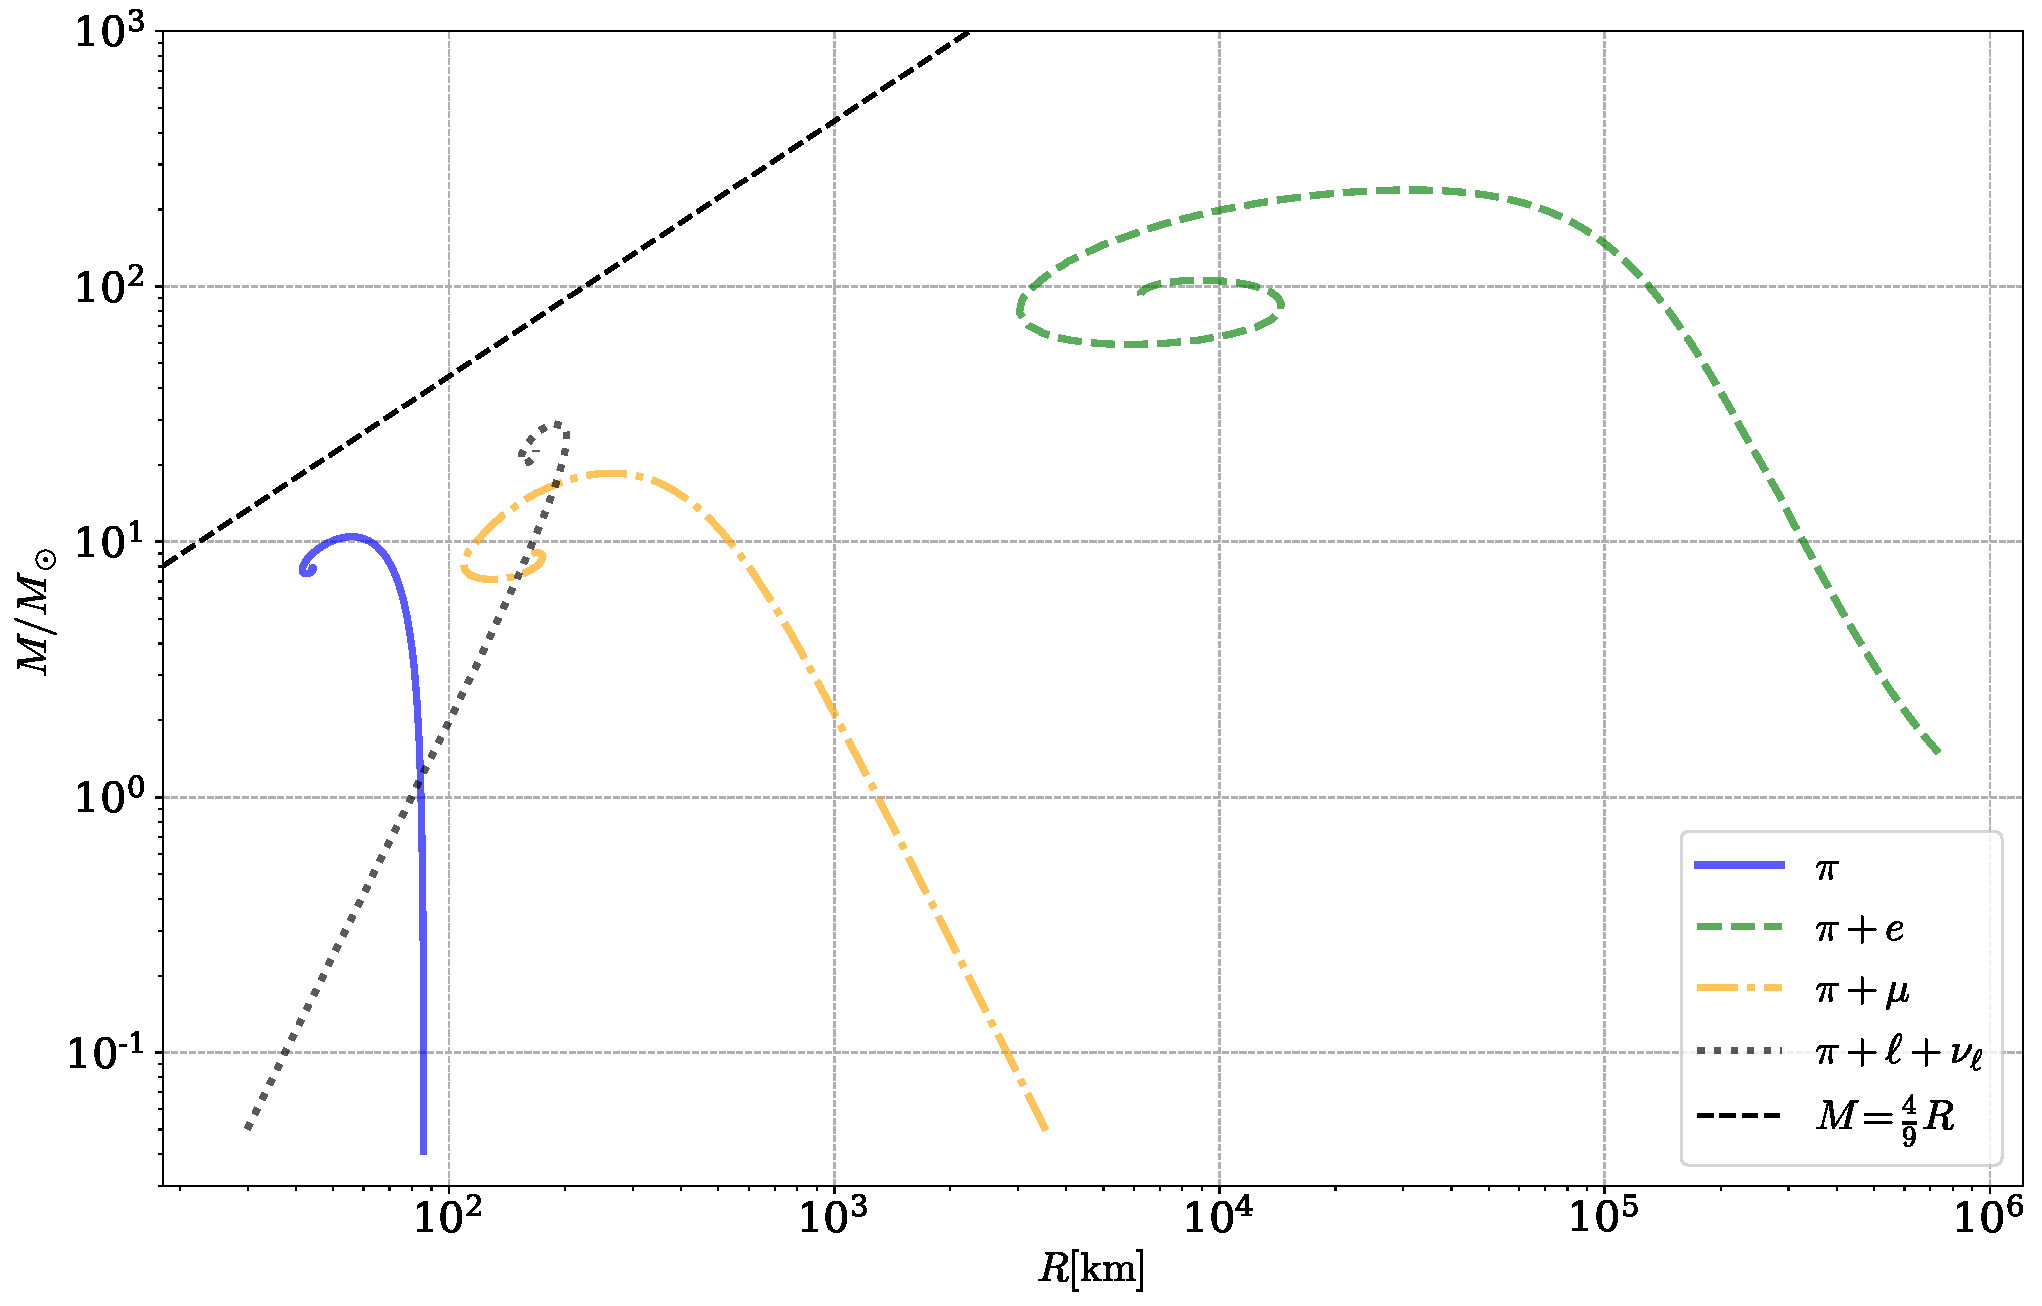
\includegraphics[width=.85\textwidth]{../scripts/figurer/pion_star/mass_radius_all.pdf}
    \caption{
        The mass-radius relations of pion stars of various compositions are compared.
        The radius is given in kilometers and the mass in units of solar masses.
        }
        \label{fig: mass-radius relation with leptons}
\end{figure}

\begin{figure}[p]
    \centering
    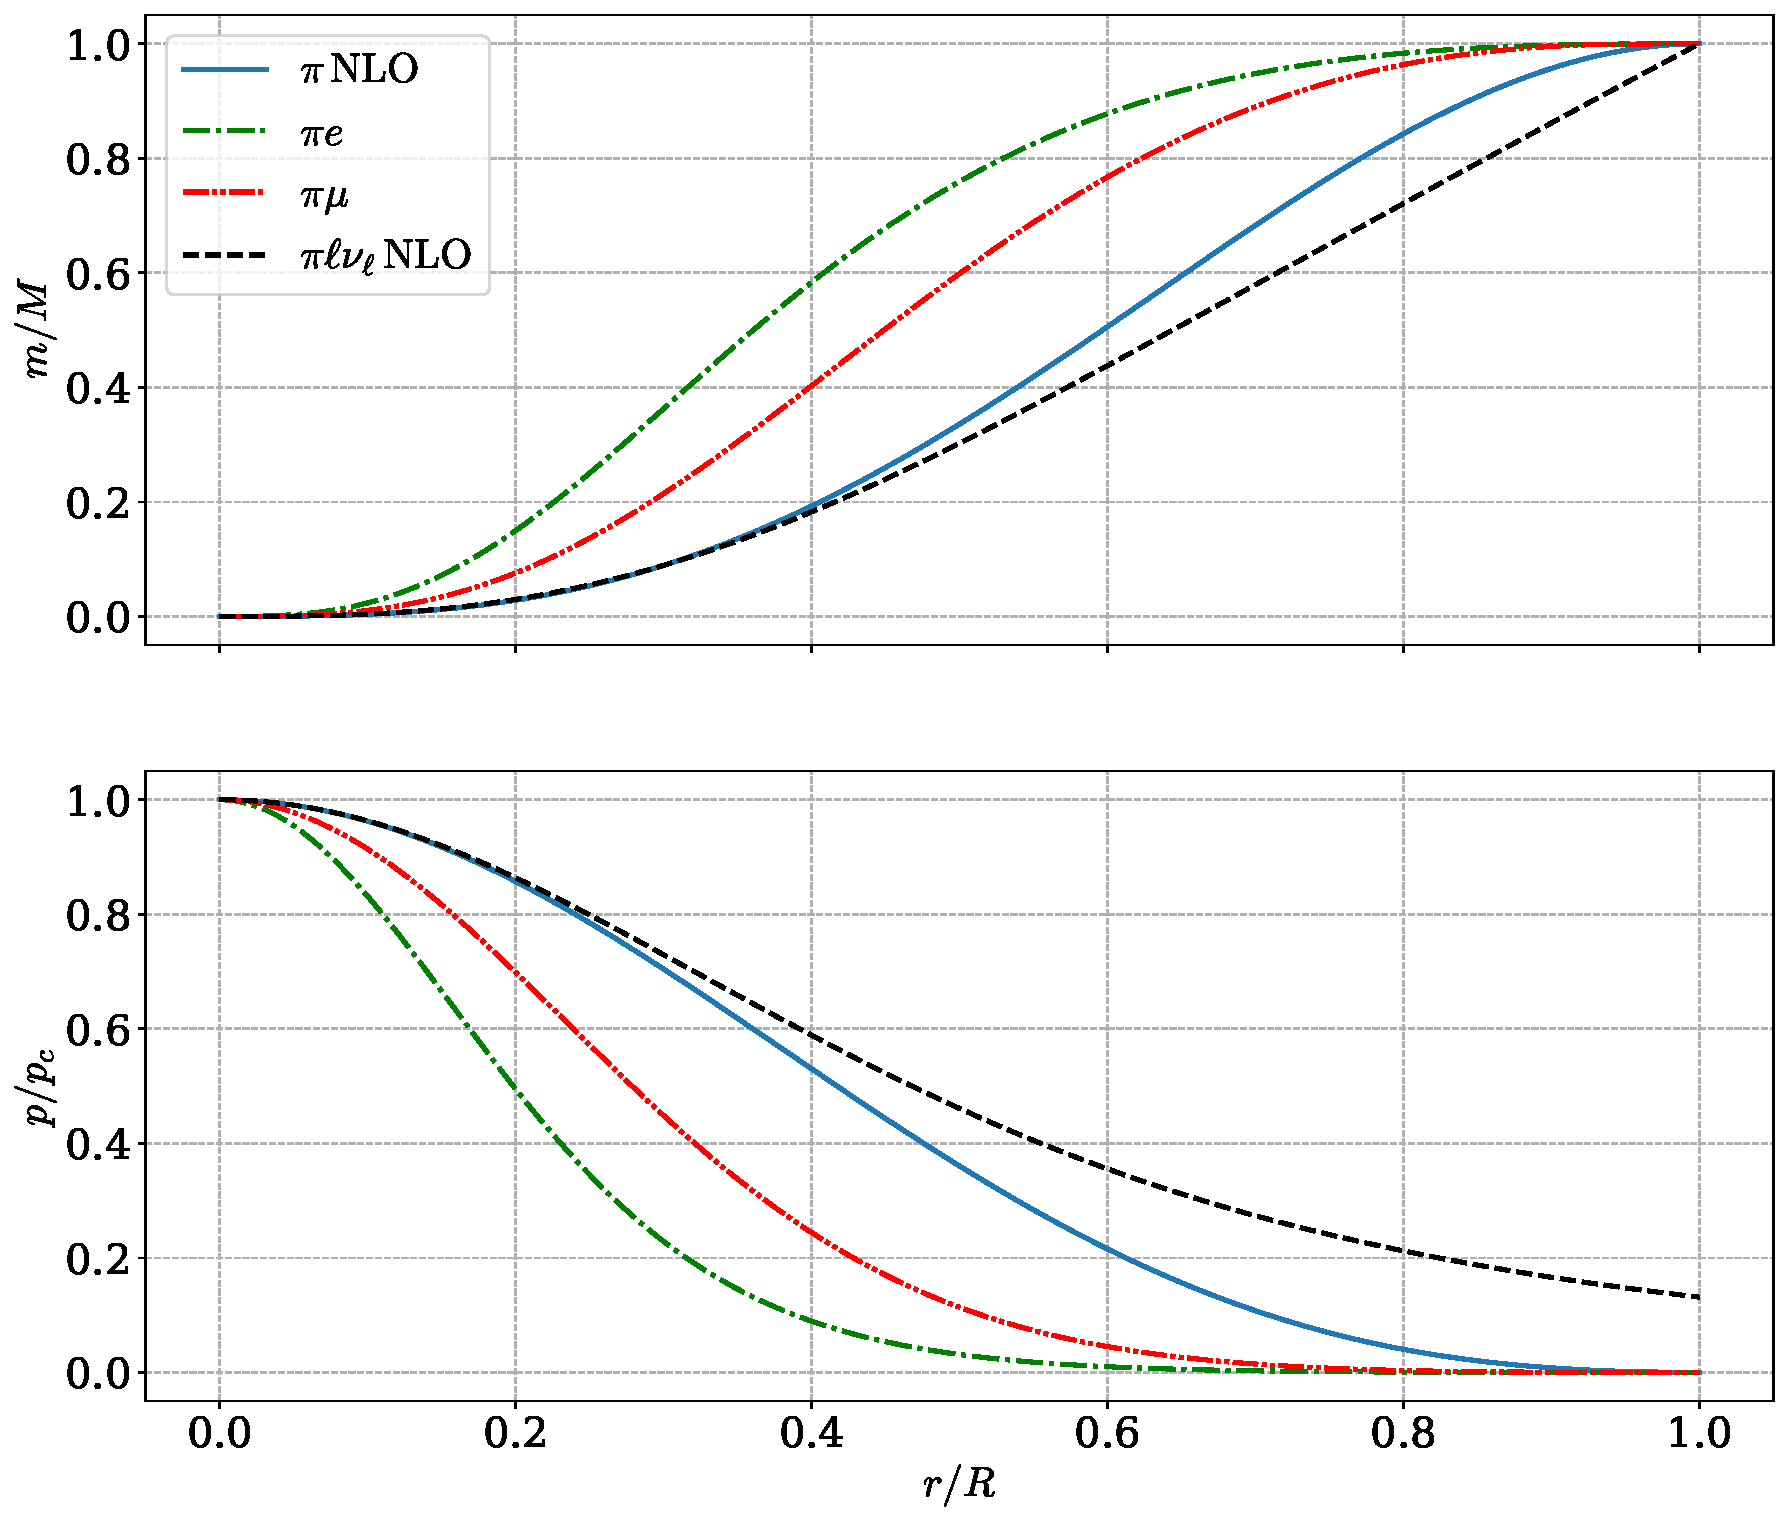
\includegraphics[width=.85\textwidth]{../scripts/figurer/pion_star/max_pressure_mass.pdf}
    \caption{
        The pressure and mass of the maximum-mass configuration of pion stars of various compositions.
        The mass, pressure, and radius are normalized to the star's stellar mass, central pressure and stellar radius.
        }
        \label{fig: max pressure and mass}
\end{figure}






\section{Comparison with QCD-lattice results}


In this section, we compare our results with earlier results obtained using lattice QCD methods.
These are first-principle numerical methods that use QCD directly without any assumption of symmetry breaking or the construction of an effective theory.
The results of \citeauthor{brandtNewClassCompact2018} for the equation of state of the pion condensate and the system with pions and electrons or muons, presented in~\autocite{brandtNewClassCompact2018}, are shown and compared with our results in \autoref{fig: brandt eos}.
With these equations of state, they obtained the mass-radius relations of pion stars.
We compare our results for the various mass-radius relations with theirs, including uncertainties, in \autoref{fig: brandt mass-radius}. 

\citeauthor{brandtNewClassCompact2018} do not use the values of physical constants from the Particle Data Group (PDG) \autocite{particledatagroupReviewParticlePhysics2020}, as we have used in this thesis.
Instead, they use the central values~\autocite{adhikariQuarkPionAxial2021}
%
\begin{align}
    m_\pi &= 131\,\text{MeV},\\
    f_\pi &= 90.5\,\text{MeV},\\
    m_K &= 481\,\text{MeV}.
\end{align}
%
Changing these constants will shift the equations of state, and consequently the mass-radius relations.
To leading order, the energy density and pressure of the pure pion condensate are
%
\begin{equation}
    \frac{p}{p_0} = \frac{1}{2} \left(\frac{\mu_I}{m_\pi} - \frac{m_\pi}{\mu_I}\right)^2,
    \quad
    \frac{u}{u_0}
    = \frac{1}{2} \left(2 + \frac{\mu_I^2}{m_\pi^2} - 3\frac{m_\pi^2}{\mu_I^2}\right).
\end{equation}
%
The change in constants therefore only leads to a scaling of the equation of state, and consequently a scaling of the mass-radius relations.
The dependence of the characteristic radius and mass on the energy density is
%
\begin{equation}
    r_0 \propto m_0 \propto \frac{1}{\sqrt{u_0}} = \frac{1}{m_\pi f_\pi}.
\end{equation}
%
As a result, $r_0$ and $m_0$ increase about $5\%$ if we use the lattice constants instead of those from the PDG.
When including other leptons and thus other mass scales or higher-order corrections, the exact effect of changing these constants becomes more complicated than a simple scaling, as there are more mass scales.
However, the magnitude of the shift is similar.
In \autoref{fig: different constants compare}, we compare both leading order and next-to-leading order results using both the constants from the PDG and those used by \citeauthor{brandtNewClassCompact2018}.
On the top are the results of the pure pion condensate and on the bottom the $\pi\ell\nu_\ell$-system.
These results are compared with the those of \citeauthor{brandtNewClassCompact2018} from \autocite{brandtNewClassCompact2018}.
In all cases, we see that lowering constants results in larger and heavier stars.

There is, in general, good agreement between the results of \citeauthor{brandtNewClassCompact2018} and our results.
In the case of the pure pion-condensate using lattice constants, we see that the next-to-leading order result is a significantly better fit than the leading order results, at least for $p<0.5 u_0$.
This is within the region where we noted chiral perturbation theory seems to converge quickly.
The different constants here do not affect the results significantly, as we compared normalized pressure and energy density.
For the mass-radius relation of the pure pion star, we see that the next-to-leading order results using the constants from the lattice simulation are in very good agreement with the numerical results, and are a significant improvement over the leading order results.
The fact that the results using the PDG constants become a less good fit from LO to NLO suggests that the lattice constants give a better comparison.
In the case of the $\pi\ell\nu_\ell$-system, the results using lattice constants are the best fit.
Here, the leading order results alone are in good agreement as the neutrino is dominating.
There is a modest improvement in the agreement at the next-to-leading order.

\clearpage

\begin{figure}[p]
    \centering
    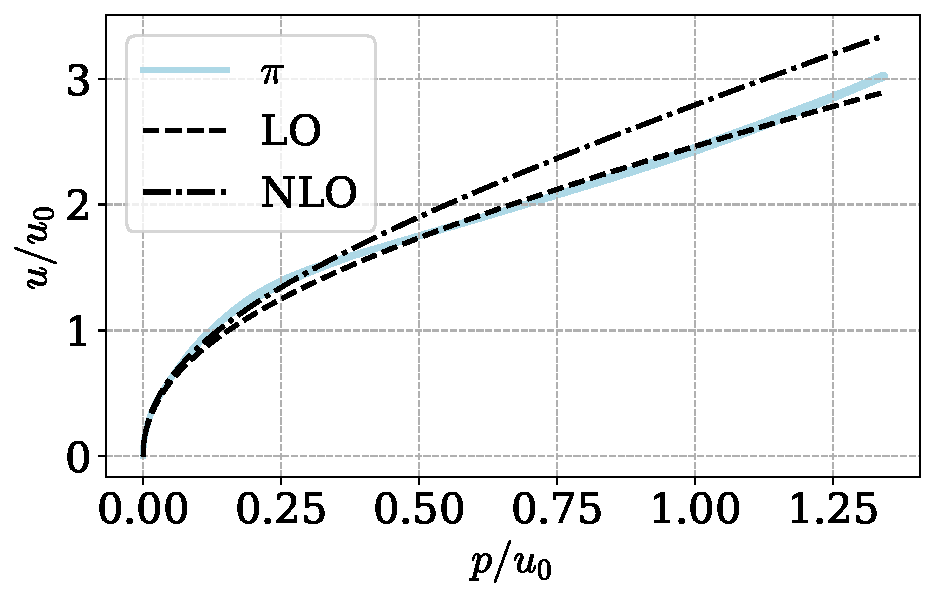
\includegraphics[width=.45\textwidth]{../scripts/figurer/brandt_eos.pdf}
    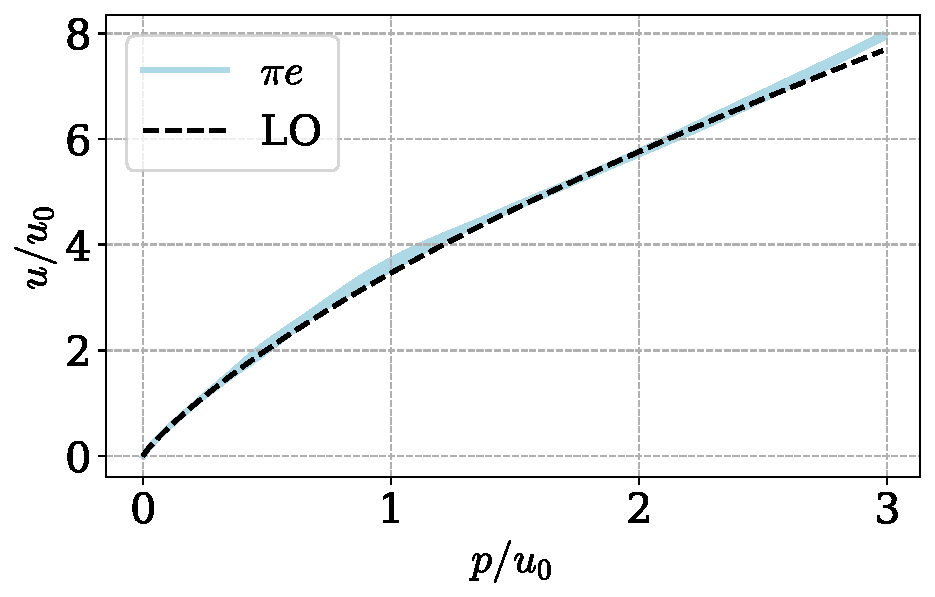
\includegraphics[width=.45\textwidth]{../scripts/figurer/brandt_eos_e.pdf}
    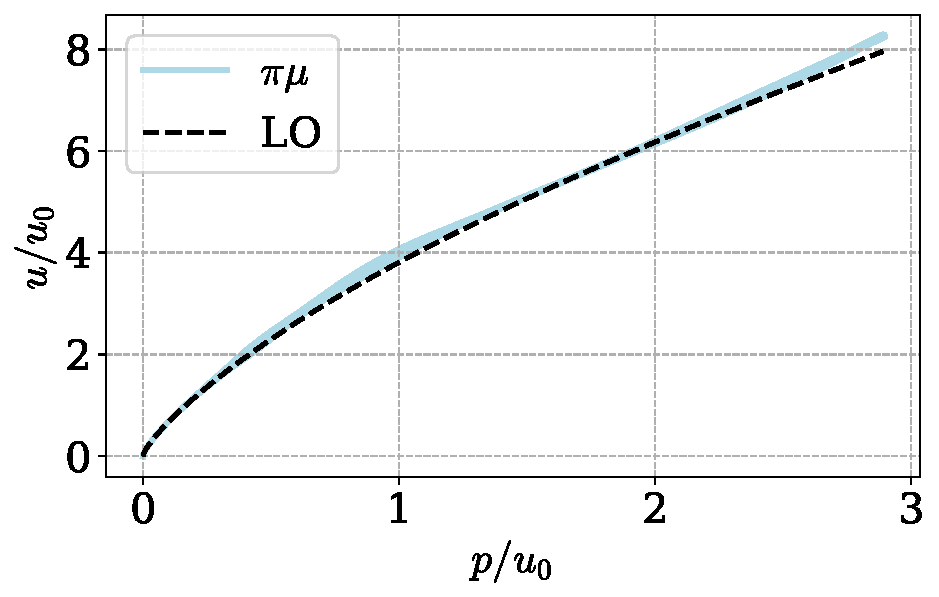
\includegraphics[width=.45\textwidth]{../scripts/figurer/brandt_eos_mu.pdf}
    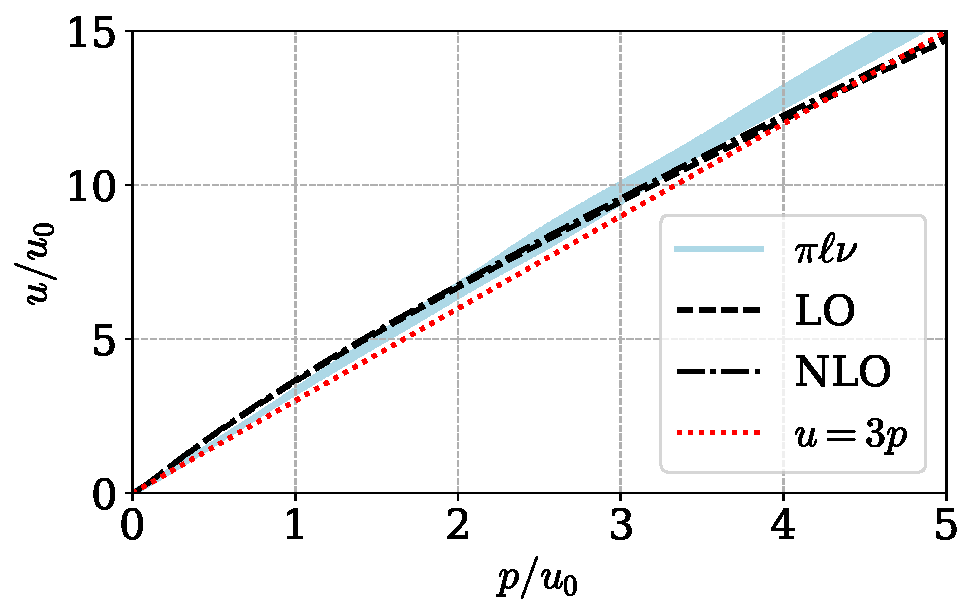
\includegraphics[width=.48\textwidth]{../scripts/figurer/brandt_eos_neutrino.pdf}
    \caption{
        The equation of state of the pion condensate with and without charged leptons.
        The results of \citeauthor{brandtNewClassCompact2018}, in solid color incorporating uncertainty, are compared to the results presented in \autoref{chapter: thermodynamics}.
        Both energy density and pressure are shown in units of $u_0 = f_\pi^2 m_\pi^2$.
        The data was provided by the authors~\autocite{brandtNewClassCompact2018}.
    }
    \label{fig: brandt eos}
\end{figure}

\begin{figure}[p]
    \centering
    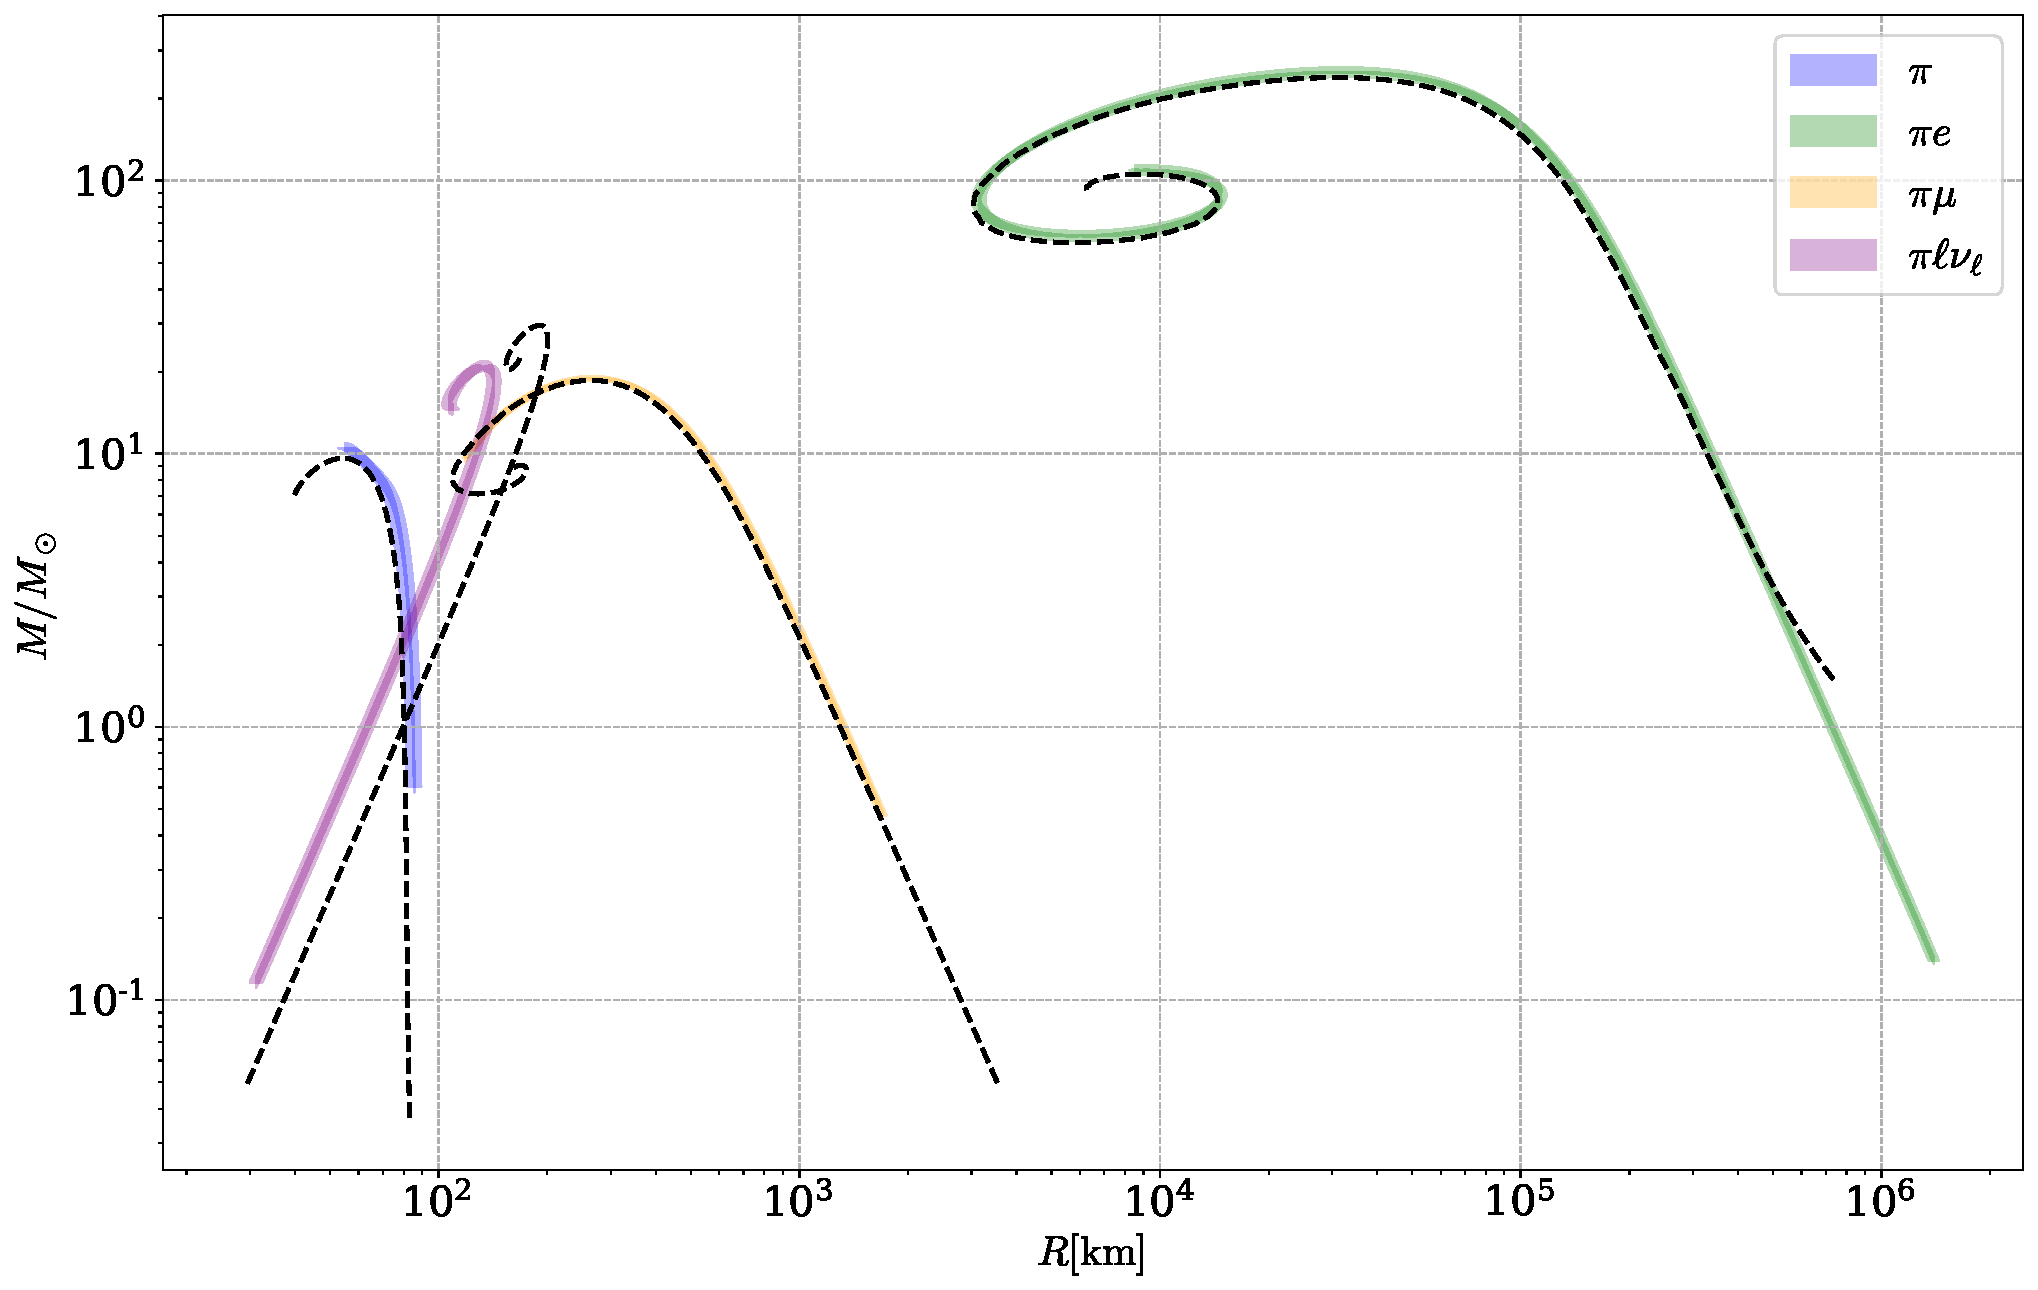
\includegraphics[width=.85\textwidth]{../scripts/figurer/pion_star/mass_radius_brandt_all.pdf}
    \caption{
        The mass-radius relations for the various pion stars.
        The results of \citeauthor{brandtNewClassCompact2018}, solid color incorporating uncertainty, are compared with our LO results, dashed lines.
        The radius is in units of $\text{km}$, while mass is in solar masses, $M_\odot$.
        The data was provided by the authors~\autocite{brandtNewClassCompact2018}.
    }
    \label{fig: brandt mass-radius}
\end{figure}


\begin{figure}[p]
    \centering
    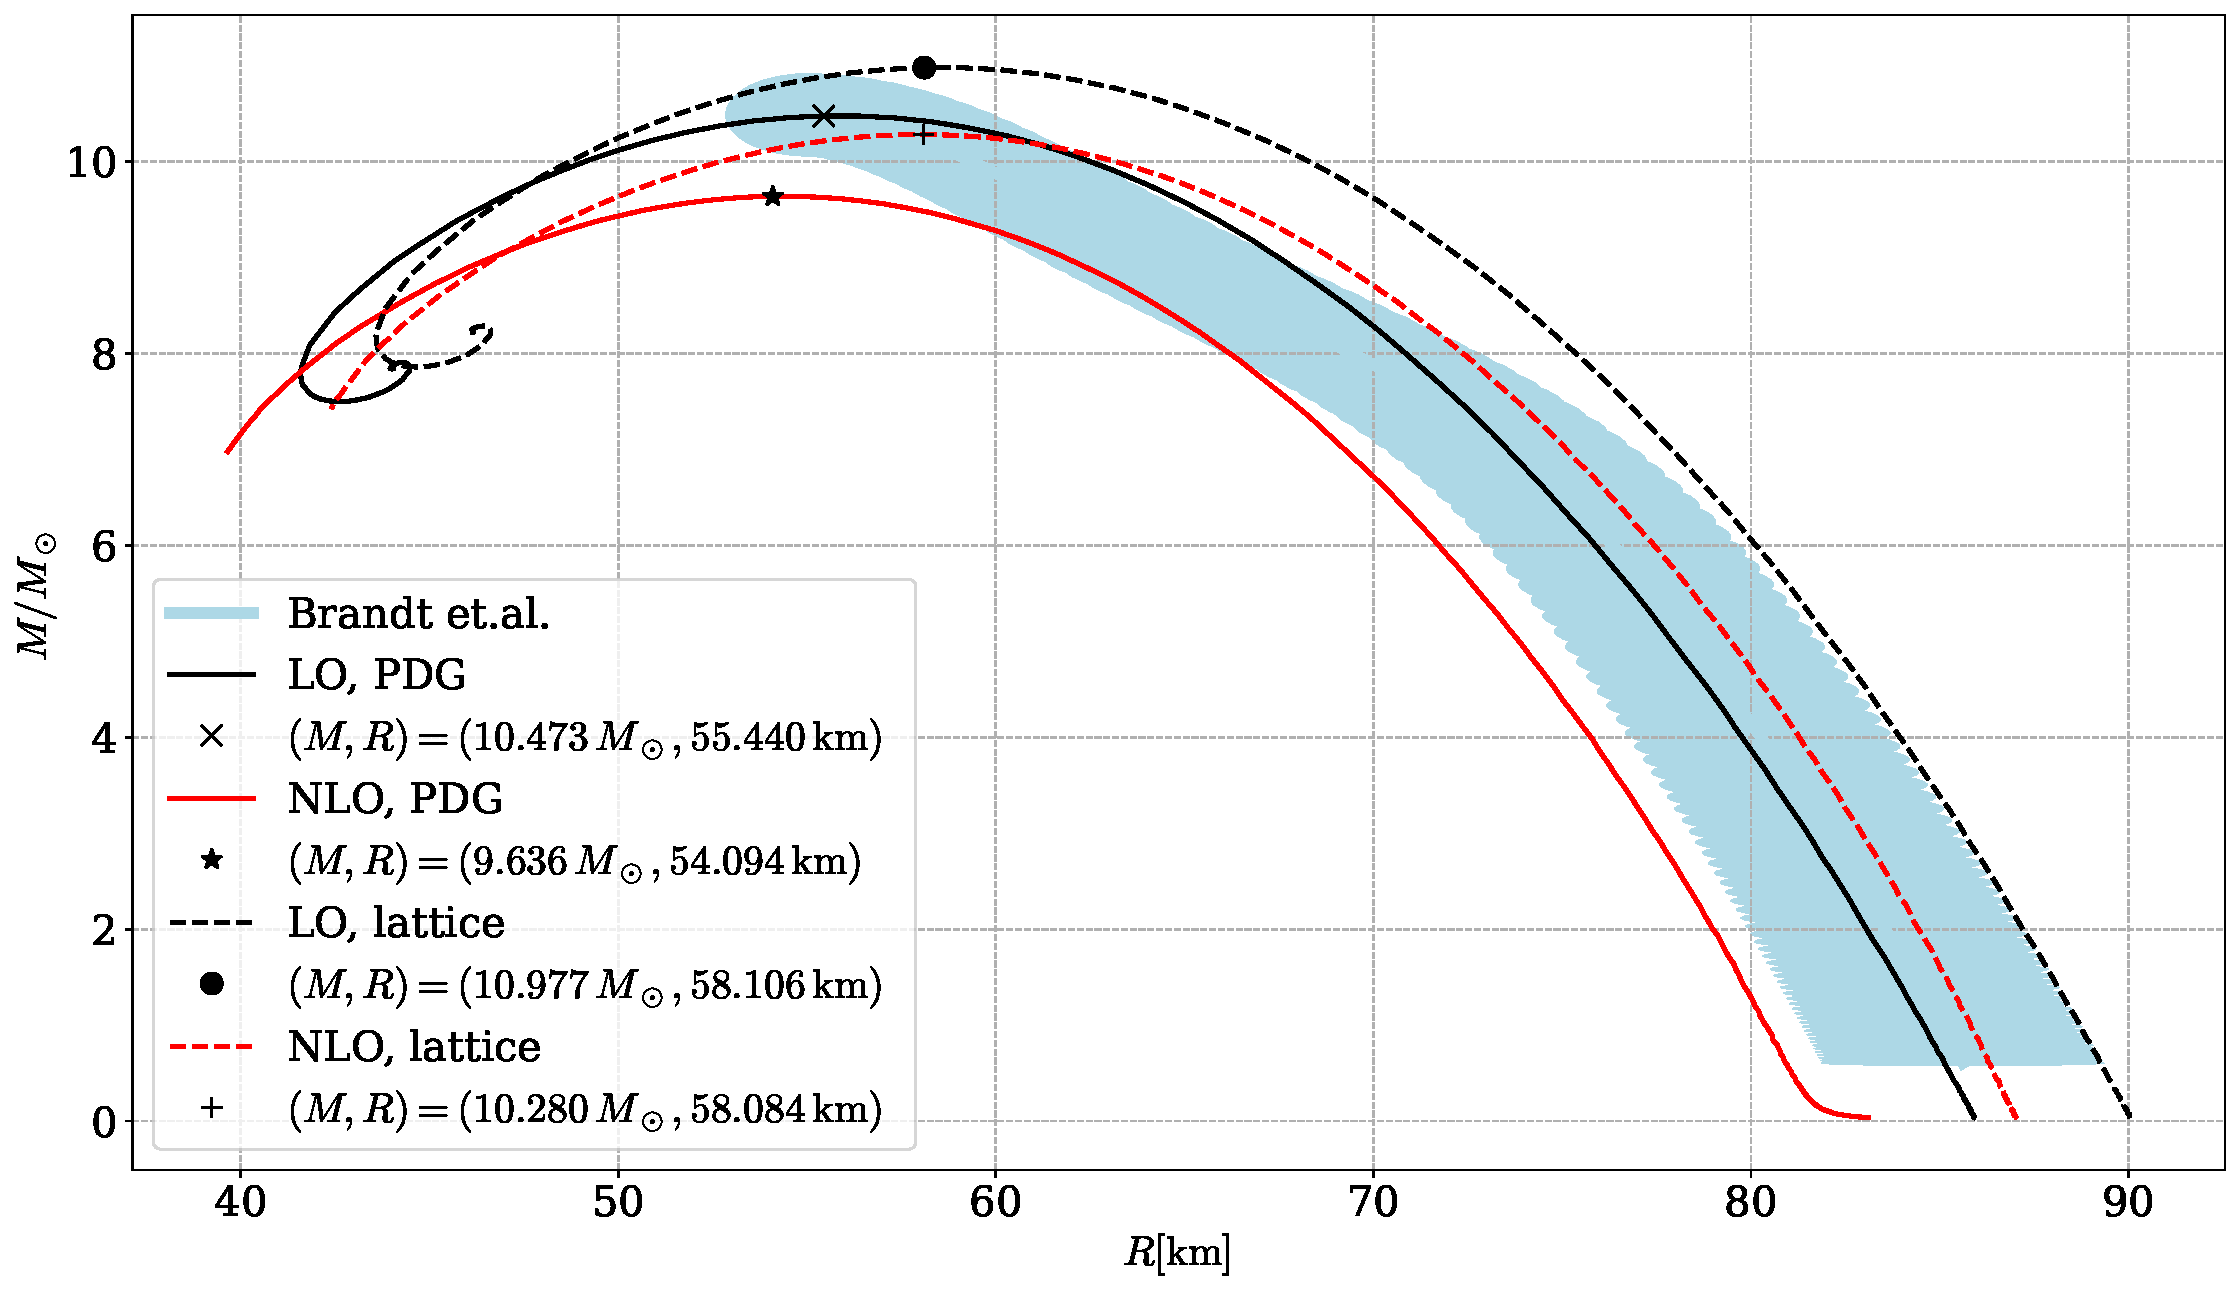
\includegraphics[width=.95\textwidth]{../scripts/figurer/pion_star/lattice_const_compare.pdf}
    \vspace{1cm}
    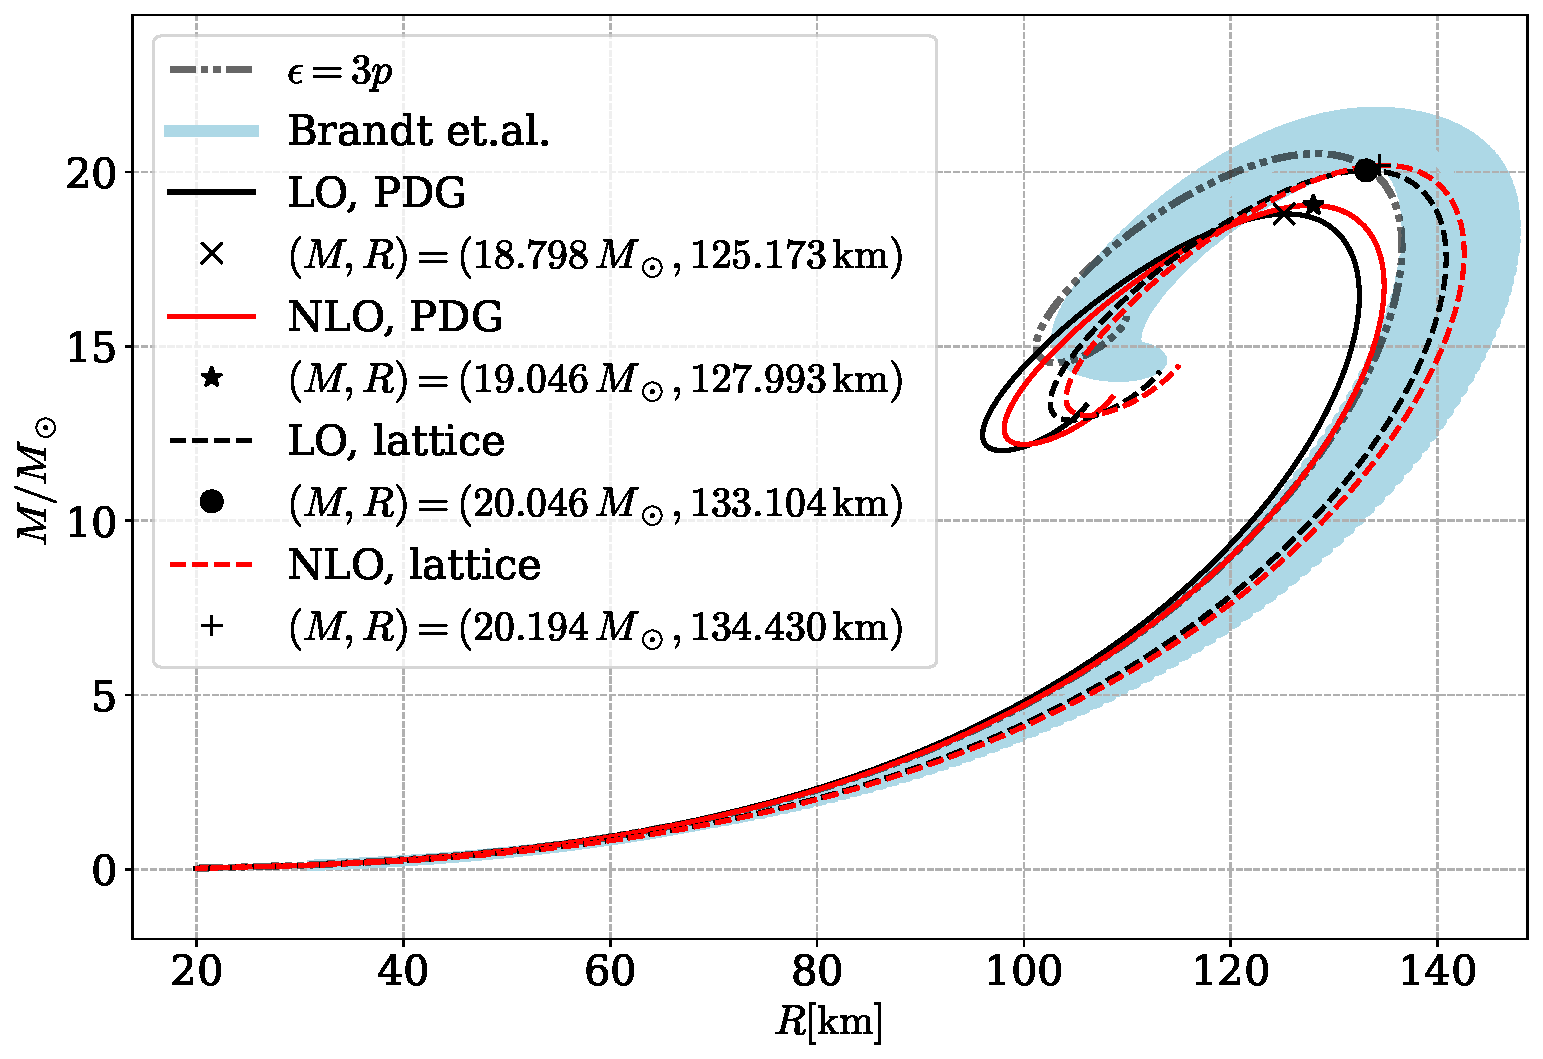
\includegraphics[width=.95\textwidth]{../scripts/figurer/pion_star/lattice_const_compare_neutrino.pdf}
    \caption{
        The mass-radius relations, using the constants from the PDG \autocite{particledatagroupReviewParticlePhysics2020} or as used in lattice QCD calculations \autocite{brandtNewClassCompact2018}.
    The results are compared with the results of \autocite{brandtNewClassCompact2018}.
    On the top are the results from a pure pion condensate, while at the bottom are the results of the $\pi\ell\nu_\ell$-system.
    }
    \label{fig: different constants compare}
\end{figure}
